\section{Topological Hochschild homology of $ku$}
\label{chap:thhkucomplet}

Here we finish the computation of $\THH_*(ku)$. We will see that $u^{p-2}\sigma u$ is indeed a class of $\THH_{2p-1}(ku;ku/v_1)$ that can be compared to $\sigma v_1 \in \THH_*(\ell;H\Z_{(p)})$. We compute $\THH_*(ku;ku/v_1)$ in \cref{section:thhkuv1} using a comparison between the Brun spectral sequences \eqref{ss:lZ} and \eqref{ss:uTB} and the truncated Bockstein spectral sequence \eqref{ss:uT} -- which has fewer classes and is easier to track.

The techniques we developed in \cref{chap:truncated} can then be used to determine the $u$-Bockstein spectral sequence for $ku$, which is done in \cref{section:thhku}. We can compare the $v_1$-Bockstein spectral sequences \eqref{ss:l} and \eqref{ss:v1}, and the Bockstein spectral sequence \eqref{ss:u} can be recovered from the truncated Bockstein spectral sequence \eqref{ss:uT} and the gathered Bockstein spectral sequence \eqref{ss:v1}.

Lastly, the extensions can be computed from the differentials and bidegree constraints of the Bockstein spectral sequence \eqref{ss:u}, thus determining $\THH_*(ku)$ as $ku_*$-module.

Our $S$-algebra model for the quotient of $ku$ by $v_1$ will be
\begin{equation}
  ku/v_1 = ku\wedge_\ell H\Z_{(p)}
\end{equation}
which is also a $q$-cofibrant commutative $S$-algebra by remark VII.6.8 of \cite{elmendorf1997rings}.

\subsection{Computation of $\THH_*(ku;ku/v_1)$}
\label{section:thhkuv1}

We will now compute $\THH_*(ku;ku/v_1)$ using both a Brun spectral sequence and a Bockstein spectral sequence. The following results allow us to compute the first page of the Brun spectral sequences.
\begin{lemma}
  \begin{enumerate}[(a)]
  \item   $(ku/v_1\wedge_{ku} ku/v_1)_*\cong P_{p-1}(u)\otimes E(\sigma v_1)$ over $\Z_{(p)}$ with $|u|=2$ and $|\sigma v_1| = 2p-1$.
  \item   $V(0)_*(ku/v_1\wedge_{ku} ku/v_1)\cong P_{p-1}(u)\otimes E(\sigma v_1)$ over $\F_p$ with $|u|=2$ and $|\sigma v_1| = 2p-1$.
  \item $\THH_*(ku/v_1;H\Z_{(p)})\cong \THH_*(H\Z_{(p)})\otimes E(\sigma u) \otimes \Gamma(\varphi u)$ over $\Z_{(p)}$ with $|\sigma u|=3$ and $|\varphi u|=2p$.
  \item $\THH_*(ku/v_1;H\F_p)\cong V(0)_*\THH(H\Z_{(p)})\otimes E(\sigma u) \otimes \Gamma(\varphi u)$ over $\F_p$ with $|\sigma u|=3$ and $|\varphi u|=2p$.
  \end{enumerate}
\end{lemma}

\begin{proof}
  The Künneth spectral sequence computing $(ku/v_1\wedge_{ku} ku/v_1)_*$ has $E^2$-page $\operatorname{Tor}^{P(u)}_{*,*}(P_{p-1}(u),P_{p-1}(u)) = P_{p-1}(u)\otimes E(\sigma v_1)$ with $|u|=(0,2)$ and $|\sigma v_1|=(1,2p-2)$. For degree reasons, the spectral sequence collapse with no possible extensions, yielding $(a)$. Point $(b)$ follows from the absence of $p$-torsion.

  We use the Brun spectral sequence to compute $\THH_*(ku/v_1;H\Z_{(p)})$ and $\THH_*(ku/v_1;H\F_p)$:
  \begin{equation}
    \THH_*(H\Z_{(p)}; H(H\Z_{(p)}\wedge_{ku/v_1} H\Z_{(p)})_*) \Rightarrow \THH_*(ku/v_1;H\Z_{(p)})
  \end{equation}
  \begin{equation}
    \THH_*(H\F_p; H(H\F_p\wedge_{ku/v_1} H\F_p)_*) \Rightarrow \THH_*(ku/v_1;H\F_p) .
  \end{equation}

  The Künneth spectral sequence computing $(H\Z_{(p)}\wedge_{ku/v_1} H\Z_{(p)})_*$ has $E^2$-page $\operatorname{Tor}^{P_{p-1}(u)}_{*,*}(\Z_{(p)},\Z_{(p)})\cong E(\sigma u)\otimes \Gamma(\varphi u)$ with $|\sigma u|=(1,2)$ and $|\varphi u|=(2,2p-2)$. The indecomposables are $\sigma u$ and the divided power $\gamma_{p^i}\varphi u$. For bidegree reasons, they cannot support non-zero differentials, so the spectral sequence collapse with no possible extensions, and we have $(H\Z_{(p)}\wedge_{ku/v_1}H\Z_{(p)})_*\cong E(\sigma u) \otimes \Gamma(\varphi u)$. A similar argument yields $(H\F_p\wedge_{ku/v_1} H\F_p)_*\cong  E(\sigma u) \otimes \Gamma(\varphi u)$, this time over $\F_p$.

  Getting back to the Brun spectral sequences, when looking at the bidegrees modulo $2p$, we see that the indecomposables also cannot support non-zero differentials in both the integral and $V(0)$ case, so that the two spectral sequences collapse. The modulo $p$ $E^\infty$-page has exactly the right rank over $\F_p$ to fit into a long exact sequence of the multiplication by $p$ for the integral $E^\infty$-page. Having an extension in the integral spectral sequence would then mean that there is a non-zero differential in the modulo $p$ one. We conclude that there is no extension in the integral spectral sequence, and $(c)$ is proven. The modulo $p$ spectral sequence cannot have extensions, and we get $(d)$.
\end{proof}

We can write the following two spectral sequences computing $\THH$ of $ku$ with coefficients in $ku/v_1$. The first one, \eqref{ss:uT}, is a truncated Bockstein spectral sequence:
\begin{gather}
  \THH_*(ku;H\Z_{(p)})\botimes P_{p-1}(u) \cong \THH_*(H\Z_{(p)})\otimes E(\sigma u) \botimes P_{p-1}(u) \notag \\
  \Rightarrow \THH_*(ku;ku/v_1) \tag{$u_T$}; \label{ss:uT} \\
\end{gather}
The second one, \eqref{ss:uTB}, is a Brun spectral sequence:
\begin{gather}
  \THH_*(ku/v_1;H(ku/v_1\wedge_{ku}ku/v_1)_*) \notag \\
  \cong\THH_*(H\Z_{(p)}) \otimes E(\sigma u)\otimes \Gamma(\varphi u) \botimes E(\sigma v_1) \otimes P_{p-1}(u) \notag \\
  \Rightarrow \THH_*(ku;ku/v_1) \tag{$u_{TB}$}. \label{ss:uTB} \\
\end{gather}
The bidegrees are:
\begin{equation}
  \begin{aligned}
    & |\sigma u| = (3,0) \\
    & |\varphi u| = (2p,0) \\
    & |\mu_{kp}| = (2kp-1,0) \mbox{, $k\geq 1$ the generators of $\THH_*(H\Z_{(p)})$} \\
    & |u| = (0,2) \\
    & |\sigma v_1| = (0,2p-1).
  \end{aligned}
\end{equation}

For the following lemma, we will briefly use the non-truncated $u$-Bockstein spectral sequence ($u$) computing $\THH_*(ku)$ that we will study in the next section. It links the class $\sigma v_1$ of $\THH_*(\ell)$ to a class of $\THH_*(ku)$.
\begin{lemma}\label{prop:imagesigmav1}
  The map $\THH_*(\ell)\rightarrow \THH_*(ku)$ sends $\sigma v_1$ to a non-zero class represented up to a unit by $u^{p-2}\sigma u$ in the Bockstein spectral sequence computing $\THH_*(ku)$.
\end{lemma}
\begin{proof}
  Since $L$ is the (smashing) localization of $\ell$ at the Johnson-Wilson spectrum $E(1)$, we can conclude from \cref{prop:localizationthh} that there is a weak equivalence
  \begin{equation}
    \THH(L) \simeq \THH(\ell;L) .
  \end{equation}
  Similarly, there is a weak equivalence
  \begin{equation}
    \THH(KU) \simeq \THH(ku;KU) .
  \end{equation}

  $\THH(\ell;L)$ can be computed using a periodic Bockstein spectral sequence
  \begin{equation}
    \THH_*(\ell;H\Z_{(p)}) \botimes P(v_1,v_1^{-1}) \Rightarrow \THH_*(\ell;L) \tag{$L$} \label{ss:L}
  \end{equation}
  which is entirely determined by the map $\eqref{ss:l}\rightarrow \eqref{ss:L}$. In particular, we can see that $\sigma v_1$ is a generator over $\Q$ and $P_\Q(v_1,v_1^{-1})$ of the summand $\Sigma L_\Q$ in the splitting
  \begin{equation}
    \THH(L)_p \simeq (L\vee\Sigma L_\Q)_p.
  \end{equation}

  Since the splitting on $\THH(L)$ and $\THH(KU)$ are compatible, it must be that $\sigma v_1\in \THH_{2p-1}(\ell)$ is sent to a non-zero class in $\THH_{2p-1}(ku)$. There is also a relation $p\mu_p = \sigma v_1$, so that the only possibility is that the image of $\sigma v_1$ in $\THH_{2p-1}(ku)$ is represented by $u^{p-2}\sigma$ to get both the extension with $p\mu_p$ and the splitting of $\THH(KU)$.
\end{proof}

Since $\ell/v_1$ is just $H\Z_{(p)}$, we have a morphism between the Brun spectral sequences $\eqref{ss:lZ}\rightarrow \eqref{ss:uTB}$ induced by the inclusion of the summand $i:\ell\rightarrow ku$. This allows us to prove:
\begin{proposition}\label{prop:diffin6}
  In \eqref{ss:uTB}, there are differentials
  \begin{equation}
    d^{2p-4}(\gamma_k\varphi u)=u^{p-2}\sigma u\gamma_{k-1}\varphi u
  \end{equation}
  up to a unit for all $k\geq 1$.
\end{proposition}
\begin{proof}
  In the following commutative diagram:
  \begin{equation}
    \begin{tikzcd}
      \THH(\ell) \rar["i"] \dar["f"] & \THH(ku) \dar["f"] \\
      \THH(\ell;H\Z_{(p)}) \rar["i"] & \THH(ku;ku/v_1)
    \end{tikzcd}
  \end{equation}
  we have up to units, using \cref{prop:imagesigmav1}
  \begin{equation}
    f(i(\sigma v_1)) = f(u^{p-2}\sigma u) = u^{p-2} f(\sigma u) = i(f(\sigma v_1)) = i(\sigma v_1) .
  \end{equation}

  In order for this to be possible, there must be an extension $u\cdot u^{p-3}\sigma u = \sigma v_1$ in \eqref{ss:uTB}, and it must be that $u^{p-2}\sigma u$ is either a boundary or not an infinite cycle. Since it is an infinite cycle for degree reasons, it is a boundary. The only class in degree $2p$ is $\varphi u$, so up to a unit there is a differential $d^{2p-4}(\varphi u)=u^{p-2}\sigma u$ in \eqref{ss:uTB}.

  In the divided power algebra $\Gamma(\varphi u)$, $\varphi u\,\gamma_{k-1} \varphi u = k\,\gamma_k\varphi u$. We can then prove our formula by induction on $k$, using the facts that
  \begin{equation}
    k\,d(\gamma_k\varphi u) = d(\varphi u) \gamma_{k-1}\varphi u + \varphi u\,d(\gamma_{k-1}\varphi u)
  \end{equation}
  and that $\Z_{(p)}$ is an integral domain.
\end{proof}

We can now get a description of all the differentials in the truncated Bockstein spectral sequence \eqref{ss:uT}:
\begin{proposition}\label{prop:diffin5}
  In the spectral sequence \eqref{ss:uT}, the differentials are given by the formula:
  \begin{equation}
    d^{2p-4}(\mu_{(k+1)p})=p^{\nu(k)}u^{p-2}\sigma u\,\mu_{kp},\quad k\geq 1
  \end{equation}
  up to a unit, where $\nu$ is the $p$-adic valuation.
\end{proposition}
\begin{proof}
  The differentials given are the only possible in \eqref{ss:uT} for bidegree reasons; we only need to prove that they are indeed non-zero. We now know enough about \eqref{ss:uTB} to do so.

  By looking at the degrees modulo $2p$, we can list the classes of total degree $2kp - 1$ in $E^1$ of \eqref{ss:uTB}:
  \begin{equation}
    \mu_{kp}, \quad \gamma_{k-1}\varphi u\,\sigma v_1, \quad \gamma_{k-1}\varphi u\,u^{p-2}\sigma u,  \quad \gamma_i\varphi u\,\mu_{(k-i)p},\; 1\leq i < k .
  \end{equation}

  We know the following differentials in \eqref{ss:uTB}:
  \begin{equation}
    d^{2p-4}(\gamma_i\varphi u)=u^{p-2}\sigma u\gamma_{i-1}\varphi u
  \end{equation}
  for $i\geq 1$ from \cref{prop:diffin6};
  \begin{equation}
    d^{2p-1}(\mu_{(i+1)p})=p^{\nu(i)}\sigma v_1\mu_{ip}
  \end{equation}
  from the map $\eqref{ss:lZ}\rightarrow (u_{TB})$ and \cref{prop:diffin4};

  To complete the multiplicative description, we also note that $\sigma v_1$ is an infinite cycle for bidegree reasons, and that all the degreewise possible value for $d^{2p-4}(\mu_{(k-i)p})$ results in a non-zero $d^{2p-4}(\gamma_i\varphi u\,\mu_{(k-i)p})$.

  From this description, after $d^{2p-1}$ the only generator left in $E^{2p}_{2kp-1}$ is $p\mu_{kp}$, so that $\THH_{2kp-1}(ku;ku/v_1)$ is isomorphic to $\Z/p^{\nu(k)}\Z$. This proves our claim about \eqref{ss:uT}.
\end{proof}

We will now describe $\THH_*(ku;ku/v_1)$; once again, we will use $v_0$ to denote multiplication by $p$ in the $E^\infty$-page of the spectral sequence \eqref{ss:uT}, and $p\cdot$ to denote the multiplication in the target group.
\begin{proposition}
  $\THH_*(ku;ku/v_1)$ is generated as a $\Z_{(p)}[u]/(u^{p-1})$-module by
  \begin{equation}
    \begin{gathered}
      1,\, \sigma u,\, \mu_p \\
      v_0\mu_{kp},\, u\mu_{kp},\, k\geq 2 \\
      \sigma u\mu_{kp},\, k\geq 1 
    \end{gathered}
  \end{equation}
  with the relations:
  \begin{equation}
    \begin{aligned}
      u^{p-2}\cdot\sigma u & = p\cdot \mu_p \\
      u\cdot v_0\mu_{kp} & = p\cdot u\mu_{kp},\, k\geq 2 \\
      p^{\nu(k)+1}\cdot u\mu_{kp} & = 0 ,\, k\geq 2\\
      u^{p-3}\cdot u\mu_{kp} & = 0 ,\, k\geq 2\\
      p^{\nu(k)+1}\cdot \sigma u\mu_{kp} & = 0 ,\, k\geq 2 \\
      p^{\nu(k)}\cdot v_0\mu_{kp} & = 0,\, k\geq 2\\
      p^{\nu(k)}u^{p-2}\cdot \sigma u\mu_{kp} & = 0,\, k\geq 2.
    \end{aligned}
  \end{equation}
\end{proposition}
\begin{proof}
  Except for the extension $p\cdot \mu_p = u^{p-2}\sigma u$ this is the $E^\infty$-page of \eqref{ss:uT}. This extension is present in \eqref{ss:lZ}, and since from \cref{prop:imagesigmav1} the map $i:\THH_*(\ell;H\Z_{(p)})\rightarrow \THH_*(ku;ku/v_1)$ is such that $i(\sigma v_1) = u^{p-2}\sigma u$, and $i(\mu_p)=\mu_p$, it must be that $u^{p-2}\sigma u$ is also divisible by $p$ in $\THH_{2p-1}(ku;ku/v_1)$. The only possible extension is with $\mu_p$, so we get our formula up to a unit.
\end{proof}

Without the module structure, writing all the classes, this is:
\begin{equation}
  \begin{aligned}
    & \Z_{(p)}\{1,\, u,\, \dots,\, u^{p-2},\, \sigma u,\,  u\sigma u,\, \dots,\, u^{p-2}\sigma u,\,  \mu_p\} \\
    & \oplus\bigoplus_{k\geq 1} \faktor{\Z}{p^{\nu(k)+1}}\{u\mu_{kp},\, u^2\mu_{kp},\, \dots,\, u^{p-2}\mu_{kp}\} \\
    & \oplus\bigoplus_{k\geq 1} \faktor{\Z}{p^{\nu(k)+1}}\{\sigma u\mu_{kp},\, u\mu_{kp},\, \dots,\, u^{p-3}\mu_{kp}\} \\
    & \oplus\bigoplus_{k\geq 2} \faktor{\Z}{p^{\nu(k)}}\{v_0\mu_{kp},\, u^{p-2}\sigma u\mu_{kp}\}
  \end{aligned}
\end{equation}
with relations $u^{p-2}\sigma u = p\cdot \mu_p$ and $u\cdot v_0\mu_{kp}=p\cdot u\mu_{kp}$.


\subsection{Computation of the Bockstein spectral se\-quen\-ce for $\THH_*(ku)$}
\label{section:thhku}

We know enough of these first three spectral sequences to compute the fourth:
\begin{align}
    & \THH_*(\ell;H\Z_{(p)})\botimes P(v_1) && \Rightarrow \THH_*(\ell) \tag{\ref{ss:l}} \\
    & \THH_*(ku;H\Z_{(p)})\botimes P_{p-1}(u) && \Rightarrow \THH_*(ku;ku/v_1) \tag{\ref{ss:uT}} \\
    & \THH(ku;ku/v_1)\botimes P(v_1) && \Rightarrow \THH_*(ku) \tag{$v_1$} \label{ss:v1} \\
    & \THH_*(ku;H\Z_{(p)})\botimes P(u) && \Rightarrow \THH_*(ku). \tag{$u$} \label{ss:u}
\end{align}

From the map $\THH(\ell;H\Z_{(p)})\rightarrow \THH(k;ku/v_1)$ comes a morphism of spectral sequences $\eqref{ss:l}\rightarrow \eqref{ss:v1}$, which determines some differentials in \eqref{ss:v1}. These differentials, the one computed in the previous section in \eqref{ss:uT} and the lemmas relating a spectral sequence and its truncations yield a description of the differentials in \eqref{ss:u}.

\begin{theorem}\label{prop:diffinu}
  The differentials in \eqref{ss:u} are given by the formula:
  \begin{equation}
    d^{p^{n+1}-2}(p^n\mu_{(k+1)p^{n+1}}) = ku^{p^{n+1}-2}\sigma u \mu_{kp^{n+1}},\; k\geq 0,\; n\geq 0
  \end{equation}
  up to a unit and linearity with respect to multiplication by $u$.
\end{theorem}
\begin{proof}
  Here we make good use of our results on truncated spectral sequences.

  First, the differentials in \eqref{ss:uT} from \cref{prop:diffin5} are lifted to \eqref{ss:u} using \cref{prop:totalandsmall}, that is in \eqref{ss:u} there are differentials:
  \begin{equation}
     \quad d^{2p-4}(\mu_{(k+1)p})=p^{\nu(k)}u^{p-2}\sigma u\,\mu_{kp},\quad k\geq 1 \label{eq:somediffinu}
  \end{equation}
  and the corresponding differentials obtained by multplying the source and the target by any power of $u$. These are the only differentials $d^r$ with $2\leq r\leq 2p-4$ in \eqref{ss:u} since these are the only differentials in \eqref{ss:uT}, again using \cref{prop:totalandsmall}.

  We will now use \cref{prop:totaltotruncated} and \cref{prop:truncatedtototal}. With regard to \cref{prop:truncatedtototal}, in our current computation, a statement stronger than the general case can be made. The general case would say that a differential $d(x)=y$ in \eqref{ss:v1} would result in the existence of an element $x'$ such that $d(x')=y$ in \eqref{ss:v1}, and such that this differential can be lifted to one in \eqref{ss:u}; but in \eqref{ss:v1}, each generator is alone in its bidegree, so that necessarily $x=x'$. So each differential $d(x)=y$ in \eqref{ss:v1} can really be lifted to a differential $d(x)=y$ in \eqref{ss:u}.

  Using \cref{prop:totaltotruncated}, the differentials of formula \eqref{eq:somediffinu} results in \eqref{ss:v1} in
  \begin{equation}
    d^1(u^i\mu_{(k+1)p})=p^{\nu(k)}v_1u^{i-1}\sigma u\,\mu_{kp},\quad k\geq 1,\quad 1\leq i\leq p-2
  \end{equation}
  and the corresponding differentials obtained by multiplying the source and the target by any power of $v_1$. These are the only differentials $d^{2p-2}$ in \eqref{ss:v1} since having more differentials would result in more differentials $d^r$ in \eqref{ss:u} with $2\leq r \leq 2p-4$. This gives the $E^2$-page of \eqref{ss:v1}:
  \begin{equation}
    \begin{aligned}
      \eqref{ss:v1} :\; E^2 \cong & \Z_{(p)}\{1,\, u,\, \dots,\, u^{p-2},\, \sigma u,\,  u\sigma u,\, \dots,\, u^{p-3}\sigma u,\,  \mu_p\}\otimes P(v_1) \\
                         &  \oplus\bigoplus_{k\geq 2} \faktor{\Z}{p^{\nu(k)}}\{v_0\mu_{kp}\}\otimes P_{p-1}(u)\otimes P(v_1) \\
                         & \oplus\bigoplus_{k\geq 1} \faktor{\Z}{p^{\nu(k)+1}}\{\sigma u\mu_{kp},\, u\,\sigma u\mu_{kp},\, \dots,\, u^{p-3}\sigma u\mu_{kp}\} \\
                         & \oplus\bigoplus_{k\geq 1} \faktor{\Z}{p^{\nu(k)}}\{u^{p-2}\sigma u\mu_{kp},\, v_1\sigma u\mu_{kp},\, u\,v_1\sigma u\mu_{kp},\, \dots\}.
    \end{aligned}
  \end{equation}

  We have written all the generators $v_0\mu_{kp}$ with $v_0$ because we will now account for the differentials in \eqref{ss:l} of \cref{prop:diffinell}:
  \begin{equation}
    d^{p^n+\dots +p}(p^{n-1}\cdot v_0\mu_{kp^n}) = (k-1) v_1^{p^n+\dots+p}\sigma v_1\mu_{(k-1)p^n},\; k\geq 1,\; n\geq 1.
  \end{equation}
  Because of the morphism of spectral sequence $(\ell) \rightarrow (v_1)$, that formula is also true in \eqref{ss:v1}, and from \cref{prop:truncatedtototal} we deduce the formula in \eqref{ss:u} that was claimed (which also encompass formula \eqref{eq:somediffinu}).

  It remains to prove that the classes $\sigma u \mu_{kp},\, k\geq 1$ are infinite cycles in \eqref{ss:u}. The classes $u^{p-2}\sigma u \mu_{kp^2},\,k\geq 1$ are in the image of $\eqref{ss:l}\rightarrow \eqref{ss:v1}$ and so are infinite cycles in \eqref{ss:v1}, thus also in \eqref{ss:u} by \cref{prop:nulldiffs}. Since in \eqref{ss:u} the only $u^{p-2}$-torsion is in even degree, it must be that $\sigma u \mu_{kp^2}$ are infinite cycles in \eqref{ss:u}. The remaining classes to check are the $\sigma u\mu_{kp}$ with $p$ not dividing $k$. Once again we now that these classes support no differentials of height up to $u^{p-2}$, and are of $u^{p-2}$-torsion after $d^{p-2}$ by formula \eqref{eq:somediffinu}. If some $\sigma u\mu_{kp}$ supports a non-zero differential the target must be $p^{\nu(k-i)}u^{ip+1}\mu_{(k-i)p},\, 1\leq i \leq k-1$ for degree reasons, and that target must be of $u^{p-2}$-torsion, that is to say some
  \begin{equation}
    \begin{gathered}
      p^{\nu(k-i)}u^{ip+2}\mu_{(k-i)p}, \\
      p^{\nu(k-i)}u^{ip+3}\mu_{(k-i)p}, \\
      \vdots \\
      p^{\nu(k-i)}u^{ip+p-1}\mu_{(k-i)p}
    \end{gathered}
  \end{equation}
  is already the target of a differential. But the only possible differentials still not accounted for are the one targeting $p^{\nu(k-i)}u^{ip+1}\mu_{(k-i)p},\, 1\leq i \leq k-1$, and these are of height $u^h$ with $h$ reducing to 1 modulo $p$.
\end{proof}

We can change our generators so that the differentials are not given up to a unit but exactly.
\begin{proposition} \label{prop:diffexactes}
  We can change the generators $\mu_N$ and $\sigma u\mu_N$ of $\THH_*(ku;H\Z_{(p)})$ with a multiplication by a unit so that the differentials in \eqref{ss:u} are given by the formula:
  \begin{equation}
    d^{p^{n+1}-2}(p^n\mu_{(k+1)p^{n+1}}) = p^{\nu(k)}u^{p^{n+1}-2}\sigma u \mu_{kp^{n+1}},\; k\geq 0,\; n\geq 0
  \end{equation}
\end{proposition}
\begin{proof}
  Note that we have chosen $p^{\nu(k)}$ instead of $k$, but these are the same up to a unit. We could have written the same statement with $k$.

  The differentials are making the $\mu_N$ and $\sigma u\mu_{N}$ interact, and once we have chosen a specific unit for one of them, we have to use the same unit for all their multiplication by powers of $p$. Consider the simple, unoriented graph $\mathcal{G}$ whose vertices are the $\mu_N$ and $\sigma u \mu_N$ for $N \geq 0$ divisible by $p$, with an edge $\mu_N \text{---}\sigma u\mu_{N'}$ whenever there is a differential
  \begin{equation}
    d(p^i\mu_N) = p^ju^\bullet\sigma u\mu_{N'}
  \end{equation}
  for any $i$ and $j$, up to a unit, in the spectral sequence. The graph $\mathcal{G}$ is bipartite, with classes given by the presence or absence of $\sigma u$ in the vertex name. If we prove that $\mathcal{G}$ is acyclic, then we have proven our statement. Indeed, $\mathcal{G}$ is then a collection of tree; we can choose an arbitrary root in each connected component of $\mathcal{G}$; starting from the roots, we can change each generation of the trees by a unit to get the formula we want.

  We will reason on the $p$-adic valuation of $N$ and $N'$, denoted $\nu(N)$ and $\nu(N')$. There is an edge $\mu_N \text{---}\sigma u\mu_{N'}$ in $\mathcal{G}$ if and only if there exists $(k,n) \in \N^2$ such that
  \begin{equation}
    N = (k+1)p^{n+1} \quad N' = kp^{n+1}.
  \end{equation}

  Fix $N$, $k$ and $n$ that $N = (k+1)p^{n+1}$, let $N' = kp^{n+1}$. Then
  \begin{equation}
    \nu(N') \geq \nu(N) \iff n+1 = \nu(N)
  \end{equation}
  so that there can only be one edge $\mu_N\text{---}\sigma u\mu_{N'}$ such that $\nu(N') \geq \nu(N)$.

   Fix $N'$, $k$ and $n$ that $N' = kp^{n+1}$, let $N = (k+1)p^{n+1}$. Then
  \begin{equation}
    \nu(N) \geq \nu(N') \iff n+1 = \nu(N')
  \end{equation}
  so that there can only be one edge $\sigma u\mu_{N'}\text{---}\mu_{N}$ such that $\nu(N) \geq \nu(N')$.

  Combining both case, we see that from any vertex of $\mathcal{G}$, there is exactly one edge such that the $p$-adic valuation is non-decreasing. If there were a non-trivial cycle in $\mathcal{G}$, we could extract an irreducible cycle, that goes through any edge at most one time. Such cycle would be confined to vertices whose $p$-adic valuation is constant, otherwise each edge would strictly decrease the valuation. But any vertex has at most one neighboor whose $p$-adic valuation is the same, thus $\mathcal{G}$ is acyclic.
\end{proof}

\subsection{Computing the extensions and a presentation of $\THH_*(ku)$}

We first compute the extensions in the torsion-free part of the spectral sequence, from the knowledge that the $p$-torsion and the $u$-torsion must be the same in $\THH_*(ku)$.
\begin{proposition}
  The torsion-free part of $\THH_*(ku)$ is a quotient of
  \begin{equation}
    P(u)\otimes \Z_{(p)}\{1,\,\sigma u,\, \mu_p,\,v_0\mu_{p^2},\,v_0^2\mu_{p^3},\,\dots \}
  \end{equation}
  with relations
  \begin{equation}
    p\cdot \mu_p = u^{p-2}\sigma u
  \end{equation}
  \begin{equation}
    p\cdot v_0^n\mu_{p^{n+1}} = u^{p^{n+1}-p^n}v_0^{n-1}\mu_{p^n},\, n\geq 1.
  \end{equation}
\end{proposition}
\begin{proof}
  From the differentials of \cref{prop:diffinu}, the generators written are the only one not of $u$-torsion. We already know from \cref{prop:torsioncoincide} that they must not be of $p$-torsion. We will see that it implies that the extensions given are present. The $u$-tower over 1 is in even degree, so no extension are possible with the rest of the classes. We prove the rest of our formula by induction on $n$. Let us first observe that each extension must be with an element not already divisible by $p$; otherwise if $p\cdot v_0^n\mu_{p^{n+1}}=p\cdot u^kx$ for some $k\geq 1$ and $x$, then $v_0^n\mu_{p^{n+1}} - u^kx$ would be an element of $p$-torsion, but represented by an element not of $u$-torsion in the spectral sequence, so not of $u$-torsion. Then $u^{p-2}\sigma u$ is the only choice (up to a unit) for $p\cdot \mu_{p}$. Let $n\geq 1$.  If our formula holds up to rank $n-1$, then $p\cdot v_0^n\mu_{p^{n+1}}$ could degreewise be:
  \begin{equation}
    \begin{gathered}
      u^{p^{n+1}-2}\sigma u \\
      u^{p^{n+1}-p}\mu_p \\
      u^{p^{n+1}-p^2}v_0\mu_{p^2} \\
      \vdots \\
      u^{p^{n+1}-p^n}v_0^{n-1}\mu_{p^n} \\
    \end{gathered}
  \end{equation}
  but the only one not already divisible by $p$ is $u^{p^{n+1}-p^n}v_0^{n-1}\mu_{p^n}$.
\end{proof}

We now give a presentation of the torsion. Before computing the extensions, we need to ensure that the lifts of the classes of the spectral sequence we choose have the correct properties.

\begin{lemma} \label{lem:liftinssu}
  For any $n\geq 1$, $0\leq h < n$ and $a\geq 1$, $a$ not divisible by $p$, the infinite cycle
  \begin{equation}
    p^h\sigma u \mu_{ap^n}
  \end{equation}
  of the spectral sequence \eqref{ss:u} lifts to an element
  \begin{equation}
    v_0^h\sigma u\mu_{ap^n}
  \end{equation}
  in $\THH_*(ku)$ such that
  \begin{equation} \label{eq:thhkuliftuzero}
    u^{p^{n-h}-2}\cdot v_0^h\sigma u \mu_{ap^n} = 0 
  \end{equation}
  and if $a = bp + p - 1$ for some $b \geq 1$,
  \begin{equation} \label{eq:thhkuliftpzero}
    p\cdot u^{p^n-3}\cdot \sigma u\mu_{(bp + p -1)p^n} = u^{p^{n+1} - 3} v_0^{\nu(b)}\sigma u\mu_{bp^{n+1}}
  \end{equation}
  otherwise we have
  \begin{equation} \label{eq:thhkuliftpzeronotdiv}
    p\cdot u^{p^n-3}\cdot v_0^h\sigma u\mu_{ap^n} = 0.
  \end{equation}
  Moreover, in both case, $p \cdot v_0^h\sigma u\mu_{ap^n}$ and $v_0^{h + 1}\sigma u \mu_{ap^n}$ differ only by an element divisible by $u$.
\end{lemma}

\begin{proof}
  We see these relations in the exact couple defining the spectral sequence \eqref{ss:u}. Since there are differentials
  \begin{equation}
    d^{p^{n+1}-2}(p^n\mu_{(k+1)p^{n+1}}) = p^{\nu(k)}u^{p^{n+1}-2}\sigma u \mu_{kp^{n+1}},\; k\geq 0,\; n\geq 0
  \end{equation}
  we can populate the diagram
    \begin{equation}
    \begin{tikzcd}[column sep = small]
      A \ar[rr, "u"] & & A \ar[rr, "u"] \ar[dl, "j"] & & ... \ar[rr, "u"] & & A \ar[rr, "u"] & & A \ar[dl, "j"] \\
      & B \ar[ul, "\partial"] & & &   & & & B \ar[ul, "\partial"] & \\
      & & \alpha \ar[rr, mapsto] \ar[dl, mapsto] & & ... \ar[rr, mapsto] & & \beta \ar[rr, mapsto] & & 0 \\
      & p^{\nu(k)}\sigma u\mu_{kp^{n+1}} & & &   & & & p^n\mu_{(k+1)p^{n+1}} \ar[ul, mapsto] &
    \end{tikzcd}
  \end{equation}
  where $A = \THH_*(ku)$ and $B=\THH_*(ku;H\Z_{(p)})$. Here we set $\beta = \partial(p^n\mu_{(k+1)p^{n+1}})$. The existence of the differential ensure that $\beta$ lifts $p^{n+1}-3$ times through the multiplication by $u$ map to an element $\alpha\in\THH_*(ku)$, and that $j(\alpha) = p^{\nu(k)}\sigma u \mu_{kp^{n+1}}$, that is $\alpha$ is represented by the the infinite cycle $p^{\nu(k)}\sigma u \mu_{kp^{n+1}}$ of the spectral sequence. We then name that element of $\THH_*(ku)$
  \begin{equation}
    \alpha = v_0^{\nu(k)}\sigma u\mu_{kp^{n+1}}
  \end{equation}
 which implies that
 \begin{equation}
   \begin{aligned}
     u^{p^{n+1}-3}v_0^{\nu(k)}\sigma u\mu_{kp^{n+1}} & = \beta \\
     u^{p^{n+1}-2}v_0^{\nu(k)}\sigma u\mu_{kp^{n+1}} & = 0
   \end{aligned}
 \end{equation}
 which is another way to write \cref{eq:thhkuliftuzero}.
 
 Moreover, the map $\partial$ is a map of $\Z_{(p)}$-modules. Thus,
 \begin{equation}
   \partial(p^{n+1}\mu_{(k+1)p^{n+1}}) = p\cdot \partial(p^n\mu_{(k+1)p^{n+1}}) \in \THH_*(ku).
 \end{equation}
 When $k+1$ is divisible by $p$, write $k= bp + p - 1$ so that $k+1 = (b+1)p$, the left hand side is already named
 \begin{equation}
  \partial (p^{n+1}\mu_{(b+1)p^{n+2}}) = u^{p^{n+2}-3}v_0^{\nu(b)}\sigma u \mu_{bp^{n+2}}
 \end{equation}
 and the right hand side is
 \begin{equation}
   \begin{aligned}
     p\cdot \partial(p^n\mu_{(b+1)p^{n+2}})
     & = p\cdot u^{p^{n+1} - 3}v_0^{\nu((b+1)p - 1)} \sigma u\mu_{((b+1)p - 1)p^{n+1}} \\
     & = p\cdot u^{p^{n+1} - 3}\sigma u\mu_{(bp + p - 1)p^{n+1}}
   \end{aligned}
 \end{equation}
 which yields \cref{eq:thhkuliftpzero} written with $n\geq 0$ instead of $n \geq 1$.

 If $k+1$ is not divisible by $p$, we have $p^{n+1}\mu_{(k+1)p^{n+1}} = 0$ in $\THH_*(ku;H\Z_{(p)})$ so
 \begin{equation}
   p\cdot \partial(p^n\mu_{(k+1)p^{n+1}}) = p\cdot u^{p^{n+1} - 3}v_0^{\nu(k)} \sigma u\mu_{kp^{n+1}} = 0
 \end{equation}
 which is \cref{eq:thhkuliftpzeronotdiv}.

 In both cases, we have
 \begin{equation}
   j(p\cdot v_0^h\sigma u\mu_{ap^n}) = p^{h+1}\sigma u \mu_{ap^n} = j(v_0^{h+1}\sigma u \mu_{ap^n})
 \end{equation}
 that is $p\cdot v_0^h\sigma u\mu_{ap^n}$ and $v_0^{h+1}\sigma u\mu_{ap^n}$ are represented by the same class in the spectral sequence. By exactness of the diagram their difference must be a multiple of $u$.
\end{proof}

Having constructed lifts of all the infinite cycles of torsion, we can recover the torsion extensions.
\begin{proposition}
  The torsion $ku_*$-sub-module of $\THH_*(ku)$ is presented by the classes
  \begin{equation}
    v_0^h\sigma u\mu_{ap^n}
  \end{equation}
  in degree $2ap^n+2$ where $h$, $a$ and $n$ are integers such that $h\geq 0$, $n\geq 1$, $a\geq 1$ and p does not divide $a$, together with the relations:
  \begin{enumerate}
  \item $v_0^{h} \sigma u \mu_{ap^n} = 0$ for any $a \geq 1$ not divisible by $p$, $n \geq 1$ and $h \geq n$.
  \item $u^{p^{n-h}-2}\cdot v_0^h\sigma u \mu_{ap^n} = 0$ for any $a \geq 1$ not divisible by $p$,  $n \geq 1$ and $0 \leq h \leq n - 1$.
  \item $p\cdot \sigma u \mu_{(bp+p-1)p^n} = v_0\sigma u\mu_{(bp+p-1)p^n}+u^{p^{n+1}-p^n}v_0^{\nu(b)}\sigma u \mu_{bp^{n+1}}$ for any $b\geq 1$ and any $n \geq 1$.
  \item  $p\cdot v_0^h\sigma u \mu_{ap^n} = v_0^{h+1}\sigma u \mu_{ap^n}$ for any $a \geq 1$ not divisible by $p$, $n \geq 1$ and $h\geq 1$ or $h=0$ not in case 3.
  \end{enumerate}
\end{proposition}

\begin{proof}
  The lifts of \cref{lem:liftinssu} have the claimed properties. Point 1 follows from the order with respect to multiplication by $p$ in the $E^\infty$-page of the spectral sequence. Point 2 is proven in the lemma. We need to check 3 and 4. For any integer $m$ and any $h \geq 0$, the lemma state that in $\THH_*(ku)$, $p\cdot v_0^h\sigma u\mu_m$ must be equal to $v_0^{h+1}\sigma u\mu_m + u\alpha$ for some $\alpha\in\THH_{*-2}(ku)$. 
  
  We examine claim 3. Let $b\geq 1$ and $n\geq 1$. Since
  \begin{equation}
    p\cdot u^{p^n-3}\cdot \sigma u\mu_{(bp + p -1)p^n} = u^{p^{n+1} - 3} v_0^{\nu(b)}\sigma u\mu_{bp^{n+1}}
  \end{equation}
  we must have
  \begin{equation}
    p\cdot \sigma u\mu_{(bp + p -1)p^n} = v_0\sigma u\mu_{(bp + p -1)p^n} + u^{p^{n+1} - p^n} v_0^{\nu(b)}\sigma u\mu_{bp^{n+1}} + u\alpha
  \end{equation}
  with $\alpha$ such that $u^{p^n-2} \alpha = 0$.

  We now examine claim 4. Let $a \geq 1$ not divisible by $p$, $h\geq 0$ and $n\geq 1$. As before, we must have
  \begin{equation}
    p\cdot v_0^h\sigma u\mu_{ap^n} = v_0^{h+1}\sigma u \mu_{ap^n} + u\alpha
  \end{equation}
  with $u^{p^{n-h}-2}\alpha = 0$.

  We will prove that in both cases, $\alpha$ must be zero. Since \cref{lem:liftinssu} lift all the torsion classes of the spectral sequence, $\alpha$ must be written with the elements we have lifted. Let $a \geq 1$ not divisible by $p$, $h\geq 0$ and $n\geq 1$ be fixed (for claim 3, we can set $a = bp + p -1$ and $h =0$). To write $\alpha$, we need to find $c\geq 1$ not divisible by $p$, $m\geq 1$ and $k\geq 0$ such that
  \begin{equation}\label{eq:forsTinTHHku}
    |v_0^k\sigma u\mu_{cp^m}| < |v_0^h\sigma u\mu_{ap^n}| < |u^{p^{m-k}-2}v_0^k\sigma u\mu_{cp^m}| \leq |u^{p^{n-h}-2}v_0^h\sigma u\mu_{ap^n}|
  \end{equation}
  in order for the $u$-tower above $\alpha$ to end before the $u$-tower above $v_0^h\sigma u \mu_{ap^n}$.

  Computing the degree, we get
  \begin{equation}
    \begin{gathered}
      2cp^m + 2 < 2ap^n + 2 < 2cp^m + 2 + 2(p^{m - k} - 2) < 2ap^n + 2 + 2(p^{n-h} - 2) \\
      \iff 0 < ap^n - cp^m < p^{m - k} - 2 < ap^n - cp^m + p^{n - h} - 2.
    \end{gathered}
  \end{equation}

  If $m \leq n$, dividing by $p^m$ we get
  \begin{equation}
    0 < ap^{n - m} - c < p^{-k} - 2p^{-m} < ap^{n-m}-c +p^{n-m-h} - 2p^{-m}
  \end{equation}
  which is impossible since $ap^{n-m} -c$ is an integer.

  If $m > n$, dividing by $p^n$ we get
  \begin{equation}
    \begin{gathered}
      0 < a - cp^{m -n} < p^{m - n - k} - 2p^{-n} < a - cp^{m - n} + p^{-h} - 2p^{-n} \\
      \iff 2p^{-n} < a - cp^{m -n} + 2p^{-n}< p^{m - n - k} < a - cp^{m - n} + p^{-h}.
    \end{gathered}
  \end{equation}
  so that $p^{m - n -k} \geq 1$ must be an integer since $a - cp^{m - n}$ is also an integer. But there can be no integer in the open interval $(a - cp^{m-n} + 2p^{-n}, a - cp^{m-n} + p^{-h})$.

  Then $\alpha$ must be zero. The only extensions that are possible in terms of degree are the one we have written, and then we know they happen because we know the relations at the top of the $u$-towers.
\end{proof}



From the two previous results, we can give a presentation of $\THH_*(ku)$ as a $ku_*$-module.
\begin{theorem} \label{prop:thhku}
  $\THH_*(ku)$ is a quotient of the $\Z_{(p)}[u]$-module
  \begin{multline}
   \Z_{(p)}[u]\{1,\,\sigma u,\, v_0^n\mu_{p^{n+1}},\,n\geq 0\} \\
    \oplus \Z_{(p)}[u]\{v_0^h\sigma u\mu_{ap^n},\, n\geq 1,\, a\geq 1,\, \mbox{$a$ not divisible by $p$},\, h\geq 0\}
  \end{multline}
  by the relations in the non-torsion part:
  \begin{itemize}
  \item $p\cdot \mu_p = u^{p-2}\sigma u$.
  \item $p\cdot v_0^n\mu_{p^{n+1}} = u^{p^{n+1}-p^n}v_0^{n-1}\mu_{p^n}$ for any $n\geq 1$.
  \end{itemize}
  and the relations in the torsion part:
  \begin{itemize}
  \item $v_0^{h} \sigma u \mu_{ap^n} = 0$ for any $a\geq 1$ not divisible by $p$, $n \geq 1$, and $h \geq n$.
  \item $u^{p^{n-h}-2}\cdot v_0^h\sigma u \mu_{ap^n} = 0$ for any $a \geq 1$ not divisible by $p$,  $n\geq 1$, and $0 \leq h \leq n - 1$.
  \item $p\cdot \sigma u \mu_{(bp+p-1)p^n} = v_0\sigma u\mu_{(bp+p-1)p^n}+u^{p^{n+1}-p^n}v_0^{\nu(b)}\sigma u \mu_{bp^{n+1}}$ for any $b\geq 1$ and any $n\geq 1$.
  \item $p\cdot v_0^h\sigma u \mu_{ap^n} = v_0^{h+1}\sigma u \mu_{ap^n}$ for any $a\geq 1$ not divisible by $p$, $n\geq 1$ and $h\geq 1$ or $h=0$ not in the previous case.
  \end{itemize}
  The degrees are:
  \begin{equation}
    \begin{aligned}
      & |\mu_{kp}| = 2kp - 1 \\
      & |\sigma u| = 3 \\
      & |v_0| = 0 \\
      & |u| = 2
    \end{aligned}
  \end{equation}
  and $\nu$ is the $p$-adic valuation.
\end{theorem}

As studied in \cite{angeltveit2010topological} for $\THH_*(\ell)$, the torsion modules of $\THH_*(ku)$ are divided into periodic submodules $T_n$ for $n\geq 1$. Each $T_n$ correspond to the submodules of the torsion elements of degrees between $|\sigma u \mu_{p^n}|= 2p^n+2$ and $|\sigma u\mu_{2p^n}| - 1 = 2(2p^n) +1$. Each of these appears $p-1$ times, by replacing the leftmost class with $\sigma u\mu_{kp^n}$ for $1 \leq k \leq p - 1$, and $p$ copies (as submodules or quotients) of $T_n$ are present in $T_{n+1}$, so $T_n$ appears an infinite numbers of times. In the following figures, the generators are named and placed on the bottom horizontal line; the rest of the non-zero class are indicated by a $\circ$ when they come from $\THH_*(\ell)$, a $\bullet$ otherwise; going straight up indicate a multiplication by $p$, and going upward and right is a multiplication by $u$; when two lines go up from a single class, it means the multiplication by $p$ is the sum of the two elements reached. None of the named classes come from $\THH_*(\ell)$.

\begin{figure}
  \centering
  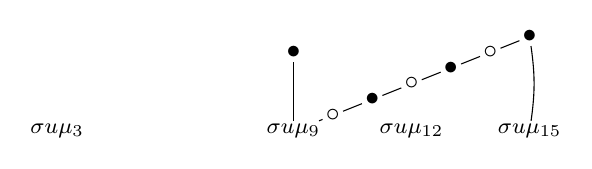
\begin{tikzpicture}
    \node[inner sep=1pt] (u0p0m3) at (-3.0,0.0) {\footnotesize$\sigma u \mu_{3}$};
    \node[inner sep=1pt] (u0p0m9) at (0.0,0.0) {\footnotesize$\sigma u \mu_{9}$};
    \node[inner sep=1pt] (u1p0m9) at (0.5,0.2) {$\circ$};
    \node[inner sep=1pt] (u2p0m9) at (1.0,0.4) {$\bullet$};
    \node[inner sep=1pt] (u3p0m9) at (1.5,0.6) {$\circ$};
    \node[inner sep=1pt] (u4p0m9) at (2.0,0.8) {$\bullet$};
    \node[inner sep=1pt] (u5p0m9) at (2.5,1.0) {$\circ$};
    \node[inner sep=1pt] (u6p0m9) at (3.0,1.2) {$\bullet$};
    \node[inner sep=1pt] (u0p1m9) at (0.0,1.0) {$\bullet$};
    \node[inner sep=1pt] (u0p0m12) at (1.5,0.0) {\footnotesize$\sigma u \mu_{12}$};
    \node[inner sep=1pt] (u0p0m15) at (3.0,0.0) {\footnotesize$\sigma u \mu_{15}$};
    \draw (u0p0m9) to (u1p0m9);
    \draw (u0p0m9) to (u0p1m9);
    \draw (u1p0m9) to (u2p0m9);
    \draw (u2p0m9) to (u3p0m9);
    \draw (u3p0m9) to (u4p0m9);
    \draw (u4p0m9) to (u5p0m9);
    \draw (u5p0m9) to (u6p0m9);
    \draw (u0p0m15) to[bend right=8] (u6p0m9);
  \end{tikzpicture}
  \caption{$T_1$ and $T_2$ for $p=3$.}
  \label{fig:p3T2}
\end{figure}

\begin{figure}
  \centering
  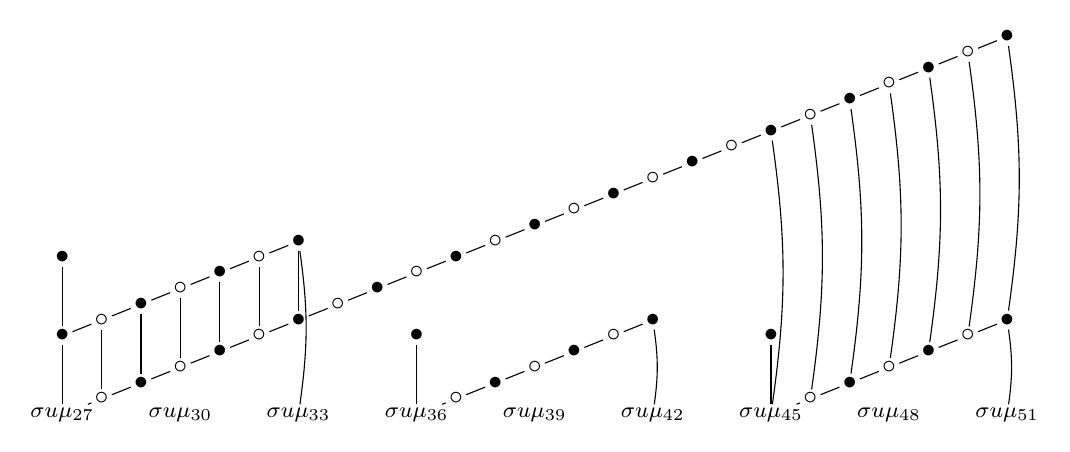
\begin{tikzpicture}
\node[inner sep=1pt] (u0p0m27) at (0.0,0.0) {\footnotesize$\sigma u \mu_{27}$};
\node[inner sep=1pt] (u1p0m27) at (0.5,0.2) {$\circ$};
\node[inner sep=1pt] (u2p0m27) at (1.0,0.4) {$\bullet$};
\node[inner sep=1pt] (u3p0m27) at (1.5,0.6) {$\circ$};
\node[inner sep=1pt] (u4p0m27) at (2.0,0.8) {$\bullet$};
\node[inner sep=1pt] (u5p0m27) at (2.5,1.0) {$\circ$};
\node[inner sep=1pt] (u6p0m27) at (3.0,1.2) {$\bullet$};
\node[inner sep=1pt] (u7p0m27) at (3.5,1.4) {$\circ$};
\node[inner sep=1pt] (u8p0m27) at (4.0,1.6) {$\bullet$};
\node[inner sep=1pt] (u9p0m27) at (4.5,1.8000001) {$\circ$};
\node[inner sep=1pt] (u10p0m27) at (5.0,2.0) {$\bullet$};
\node[inner sep=1pt] (u11p0m27) at (5.5,2.2) {$\circ$};
\node[inner sep=1pt] (u12p0m27) at (6.0,2.4) {$\bullet$};
\node[inner sep=1pt] (u13p0m27) at (6.5,2.6000001) {$\circ$};
\node[inner sep=1pt] (u14p0m27) at (7.0,2.8) {$\bullet$};
\node[inner sep=1pt] (u15p0m27) at (7.5,3.0) {$\circ$};
\node[inner sep=1pt] (u16p0m27) at (8.0,3.2) {$\bullet$};
\node[inner sep=1pt] (u17p0m27) at (8.5,3.4) {$\circ$};
\node[inner sep=1pt] (u18p0m27) at (9.0,3.6000001) {$\bullet$};
\node[inner sep=1pt] (u19p0m27) at (9.5,3.8) {$\circ$};
\node[inner sep=1pt] (u20p0m27) at (10.0,4.0) {$\bullet$};
\node[inner sep=1pt] (u21p0m27) at (10.5,4.2000003) {$\circ$};
\node[inner sep=1pt] (u22p0m27) at (11.0,4.4) {$\bullet$};
\node[inner sep=1pt] (u23p0m27) at (11.5,4.6) {$\circ$};
\node[inner sep=1pt] (u24p0m27) at (12.0,4.8) {$\bullet$};
\node[inner sep=1pt] (u0p1m27) at (0.0,1.0) {$\bullet$};
\node[inner sep=1pt] (u1p1m27) at (0.5,1.2) {$\circ$};
\node[inner sep=1pt] (u2p1m27) at (1.0,1.4) {$\bullet$};
\node[inner sep=1pt] (u3p1m27) at (1.5,1.6) {$\circ$};
\node[inner sep=1pt] (u4p1m27) at (2.0,1.8) {$\bullet$};
\node[inner sep=1pt] (u5p1m27) at (2.5,2.0) {$\circ$};
\node[inner sep=1pt] (u6p1m27) at (3.0,2.2) {$\bullet$};
\node[inner sep=1pt] (u0p2m27) at (0.0,2.0) {$\bullet$};
\node[inner sep=1pt] (u0p0m30) at (1.5,0.0) {\footnotesize$\sigma u \mu_{30}$};
\node[inner sep=1pt] (u0p0m33) at (3.0,0.0) {\footnotesize$\sigma u \mu_{33}$};
\node[inner sep=1pt] (u0p0m36) at (4.5,0.0) {\footnotesize$\sigma u \mu_{36}$};
\node[inner sep=1pt] (u1p0m36) at (5.0,0.2) {$\circ$};
\node[inner sep=1pt] (u2p0m36) at (5.5,0.4) {$\bullet$};
\node[inner sep=1pt] (u3p0m36) at (6.0,0.6) {$\circ$};
\node[inner sep=1pt] (u4p0m36) at (6.5,0.8) {$\bullet$};
\node[inner sep=1pt] (u5p0m36) at (7.0,1.0) {$\circ$};
\node[inner sep=1pt] (u6p0m36) at (7.5,1.2) {$\bullet$};
\node[inner sep=1pt] (u0p1m36) at (4.5,1.0) {$\bullet$};
\node[inner sep=1pt] (u0p0m39) at (6.0,0.0) {\footnotesize$\sigma u \mu_{39}$};
\node[inner sep=1pt] (u0p0m42) at (7.5,0.0) {\footnotesize$\sigma u \mu_{42}$};
\node[inner sep=1pt] (u0p0m45) at (9.0,0.0) {\footnotesize$\sigma u \mu_{45}$};
\node[inner sep=1pt] (u1p0m45) at (9.5,0.2) {$\circ$};
\node[inner sep=1pt] (u2p0m45) at (10.0,0.4) {$\bullet$};
\node[inner sep=1pt] (u3p0m45) at (10.5,0.6) {$\circ$};
\node[inner sep=1pt] (u4p0m45) at (11.0,0.8) {$\bullet$};
\node[inner sep=1pt] (u5p0m45) at (11.5,1.0) {$\circ$};
\node[inner sep=1pt] (u6p0m45) at (12.0,1.2) {$\bullet$};
\node[inner sep=1pt] (u0p1m45) at (9.0,1.0) {$\bullet$};
\node[inner sep=1pt] (u0p0m48) at (10.5,0.0) {\footnotesize$\sigma u \mu_{48}$};
\node[inner sep=1pt] (u0p0m51) at (12.0,0.0) {\footnotesize$\sigma u \mu_{51}$};
\draw (u0p0m27) to (u1p0m27);
\draw (u0p0m27) to (u0p1m27);
\draw (u1p0m27) to (u2p0m27);
\draw (u1p0m27) to (u1p1m27);
\draw (u2p0m27) to (u3p0m27);
\draw (u2p0m27) to (u2p1m27);
\draw (u3p0m27) to (u4p0m27);
\draw (u3p0m27) to (u3p1m27);
\draw (u4p0m27) to (u5p0m27);
\draw (u4p0m27) to (u4p1m27);
\draw (u5p0m27) to (u6p0m27);
\draw (u5p0m27) to (u5p1m27);
\draw (u6p0m27) to (u7p0m27);
\draw (u6p0m27) to (u6p1m27);
\draw (u7p0m27) to (u8p0m27);
\draw (u8p0m27) to (u9p0m27);
\draw (u9p0m27) to (u10p0m27);
\draw (u10p0m27) to (u11p0m27);
\draw (u11p0m27) to (u12p0m27);
\draw (u12p0m27) to (u13p0m27);
\draw (u13p0m27) to (u14p0m27);
\draw (u14p0m27) to (u15p0m27);
\draw (u15p0m27) to (u16p0m27);
\draw (u16p0m27) to (u17p0m27);
\draw (u17p0m27) to (u18p0m27);
\draw (u18p0m27) to (u19p0m27);
\draw (u19p0m27) to (u20p0m27);
\draw (u20p0m27) to (u21p0m27);
\draw (u21p0m27) to (u22p0m27);
\draw (u22p0m27) to (u23p0m27);
\draw (u23p0m27) to (u24p0m27);
\draw (u0p1m27) to (u1p1m27);
\draw (u0p1m27) to (u0p2m27);
\draw (u1p1m27) to (u2p1m27);
\draw (u2p1m27) to (u3p1m27);
\draw (u3p1m27) to (u4p1m27);
\draw (u4p1m27) to (u5p1m27);
\draw (u5p1m27) to (u6p1m27);
\draw (u0p0m33) to[bend right=8] (u6p1m27);
\draw (u0p0m36) to (u1p0m36);
\draw (u0p0m36) to (u0p1m36);
\draw (u1p0m36) to (u2p0m36);
\draw (u2p0m36) to (u3p0m36);
\draw (u3p0m36) to (u4p0m36);
\draw (u4p0m36) to (u5p0m36);
\draw (u5p0m36) to (u6p0m36);
\draw (u0p0m42) to[bend right=8] (u6p0m36);
\draw (u0p0m45) to (u1p0m45);
\draw (u0p0m45) to (u0p1m45);
\draw (u0p0m45) to[bend right=8] (u18p0m27);
\draw (u1p0m45) to (u2p0m45);
\draw (u1p0m45) to[bend right=8] (u19p0m27);
\draw (u2p0m45) to (u3p0m45);
\draw (u2p0m45) to[bend right=8] (u20p0m27);
\draw (u3p0m45) to (u4p0m45);
\draw (u3p0m45) to[bend right=8] (u21p0m27);
\draw (u4p0m45) to (u5p0m45);
\draw (u4p0m45) to[bend right=8] (u22p0m27);
\draw (u5p0m45) to (u6p0m45);
\draw (u5p0m45) to[bend right=8] (u23p0m27);
\draw (u6p0m45) to[bend right=8] (u24p0m27);
\draw (u0p0m51) to[bend right=8] (u6p0m45);
\end{tikzpicture}
  \caption{$T_3$ for $p=3$.}
  \label{fig:p3T3}
\end{figure}

\begin{figure}
  \centering
  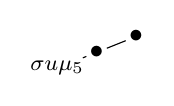
\begin{tikzpicture}
\node[inner sep=1pt] (u0p0m5) at (0.0,0.0) {\footnotesize$\sigma u \mu_{5}$};
\node[inner sep=1pt] (u1p0m5) at (0.5,0.2) {$\bullet$};
\node[inner sep=1pt] (u2p0m5) at (1.0,0.4) {$\bullet$};
\draw (u0p0m5) to (u1p0m5);
\draw (u1p0m5) to (u2p0m5);
\end{tikzpicture}
  \caption{$T_1$ for $p=5$.}
  \label{fig:p5T1}
\end{figure}

\begin{figure}
  \centering
  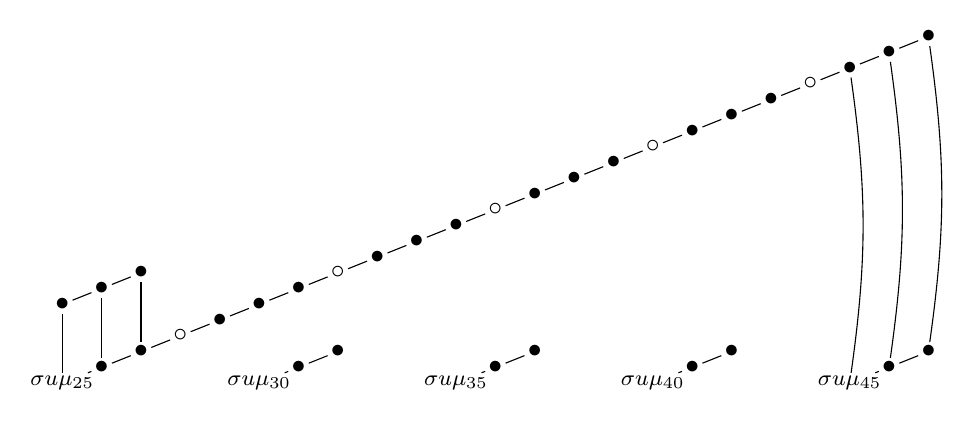
\begin{tikzpicture}
\node[inner sep=1pt] (u0p0m25) at (0.0,0.0) {\footnotesize$\sigma u \mu_{25}$};
\node[inner sep=1pt] (u1p0m25) at (0.5,0.2) {$\bullet$};
\node[inner sep=1pt] (u2p0m25) at (1.0,0.4) {$\bullet$};
\node[inner sep=1pt] (u3p0m25) at (1.5,0.6) {$\circ$};
\node[inner sep=1pt] (u4p0m25) at (2.0,0.8) {$\bullet$};
\node[inner sep=1pt] (u5p0m25) at (2.5,1.0) {$\bullet$};
\node[inner sep=1pt] (u6p0m25) at (3.0,1.2) {$\bullet$};
\node[inner sep=1pt] (u7p0m25) at (3.5,1.4) {$\circ$};
\node[inner sep=1pt] (u8p0m25) at (4.0,1.6) {$\bullet$};
\node[inner sep=1pt] (u9p0m25) at (4.5,1.8000001) {$\bullet$};
\node[inner sep=1pt] (u10p0m25) at (5.0,2.0) {$\bullet$};
\node[inner sep=1pt] (u11p0m25) at (5.5,2.2) {$\circ$};
\node[inner sep=1pt] (u12p0m25) at (6.0,2.4) {$\bullet$};
\node[inner sep=1pt] (u13p0m25) at (6.5,2.6000001) {$\bullet$};
\node[inner sep=1pt] (u14p0m25) at (7.0,2.8) {$\bullet$};
\node[inner sep=1pt] (u15p0m25) at (7.5,3.0) {$\circ$};
\node[inner sep=1pt] (u16p0m25) at (8.0,3.2) {$\bullet$};
\node[inner sep=1pt] (u17p0m25) at (8.5,3.4) {$\bullet$};
\node[inner sep=1pt] (u18p0m25) at (9.0,3.6000001) {$\bullet$};
\node[inner sep=1pt] (u19p0m25) at (9.5,3.8) {$\circ$};
\node[inner sep=1pt] (u20p0m25) at (10.0,4.0) {$\bullet$};
\node[inner sep=1pt] (u21p0m25) at (10.5,4.2000003) {$\bullet$};
\node[inner sep=1pt] (u22p0m25) at (11.0,4.4) {$\bullet$};
\node[inner sep=1pt] (u0p1m25) at (0.0,1.0) {$\bullet$};
\node[inner sep=1pt] (u1p1m25) at (0.5,1.2) {$\bullet$};
\node[inner sep=1pt] (u2p1m25) at (1.0,1.4) {$\bullet$};
\node[inner sep=1pt] (u0p0m30) at (2.5,0.0) {\footnotesize$\sigma u \mu_{30}$};
\node[inner sep=1pt] (u1p0m30) at (3.0,0.2) {$\bullet$};
\node[inner sep=1pt] (u2p0m30) at (3.5,0.4) {$\bullet$};
\node[inner sep=1pt] (u0p0m35) at (5.0,0.0) {\footnotesize$\sigma u \mu_{35}$};
\node[inner sep=1pt] (u1p0m35) at (5.5,0.2) {$\bullet$};
\node[inner sep=1pt] (u2p0m35) at (6.0,0.4) {$\bullet$};
\node[inner sep=1pt] (u0p0m40) at (7.5,0.0) {\footnotesize$\sigma u \mu_{40}$};
\node[inner sep=1pt] (u1p0m40) at (8.0,0.2) {$\bullet$};
\node[inner sep=1pt] (u2p0m40) at (8.5,0.4) {$\bullet$};
\node[inner sep=1pt] (u0p0m45) at (10.0,0.0) {\footnotesize$\sigma u \mu_{45}$};
\node[inner sep=1pt] (u1p0m45) at (10.5,0.2) {$\bullet$};
\node[inner sep=1pt] (u2p0m45) at (11.0,0.4) {$\bullet$};
\draw (u0p0m25) to (u1p0m25);
\draw (u0p0m25) to (u0p1m25);
\draw (u1p0m25) to (u2p0m25);
\draw (u1p0m25) to (u1p1m25);
\draw (u2p0m25) to (u3p0m25);
\draw (u2p0m25) to (u2p1m25);
\draw (u3p0m25) to (u4p0m25);
\draw (u4p0m25) to (u5p0m25);
\draw (u5p0m25) to (u6p0m25);
\draw (u6p0m25) to (u7p0m25);
\draw (u7p0m25) to (u8p0m25);
\draw (u8p0m25) to (u9p0m25);
\draw (u9p0m25) to (u10p0m25);
\draw (u10p0m25) to (u11p0m25);
\draw (u11p0m25) to (u12p0m25);
\draw (u12p0m25) to (u13p0m25);
\draw (u13p0m25) to (u14p0m25);
\draw (u14p0m25) to (u15p0m25);
\draw (u15p0m25) to (u16p0m25);
\draw (u16p0m25) to (u17p0m25);
\draw (u17p0m25) to (u18p0m25);
\draw (u18p0m25) to (u19p0m25);
\draw (u19p0m25) to (u20p0m25);
\draw (u20p0m25) to (u21p0m25);
\draw (u21p0m25) to (u22p0m25);
\draw (u0p1m25) to (u1p1m25);
\draw (u1p1m25) to (u2p1m25);
\draw (u0p0m30) to (u1p0m30);
\draw (u1p0m30) to (u2p0m30);
\draw (u0p0m35) to (u1p0m35);
\draw (u1p0m35) to (u2p0m35);
\draw (u0p0m40) to (u1p0m40);
\draw (u1p0m40) to (u2p0m40);
\draw (u0p0m45) to (u1p0m45);
\draw (u0p0m45) to[bend right=8] (u20p0m25);
\draw (u1p0m45) to (u2p0m45);
\draw (u1p0m45) to[bend right=8] (u21p0m25);
\draw (u2p0m45) to[bend right=8] (u22p0m25);
\end{tikzpicture}
  \caption{$T_2$ for $p=5$.}
  \label{fig:p5T2}
\end{figure}

\begin{sidewaysfigure}
  \centering
  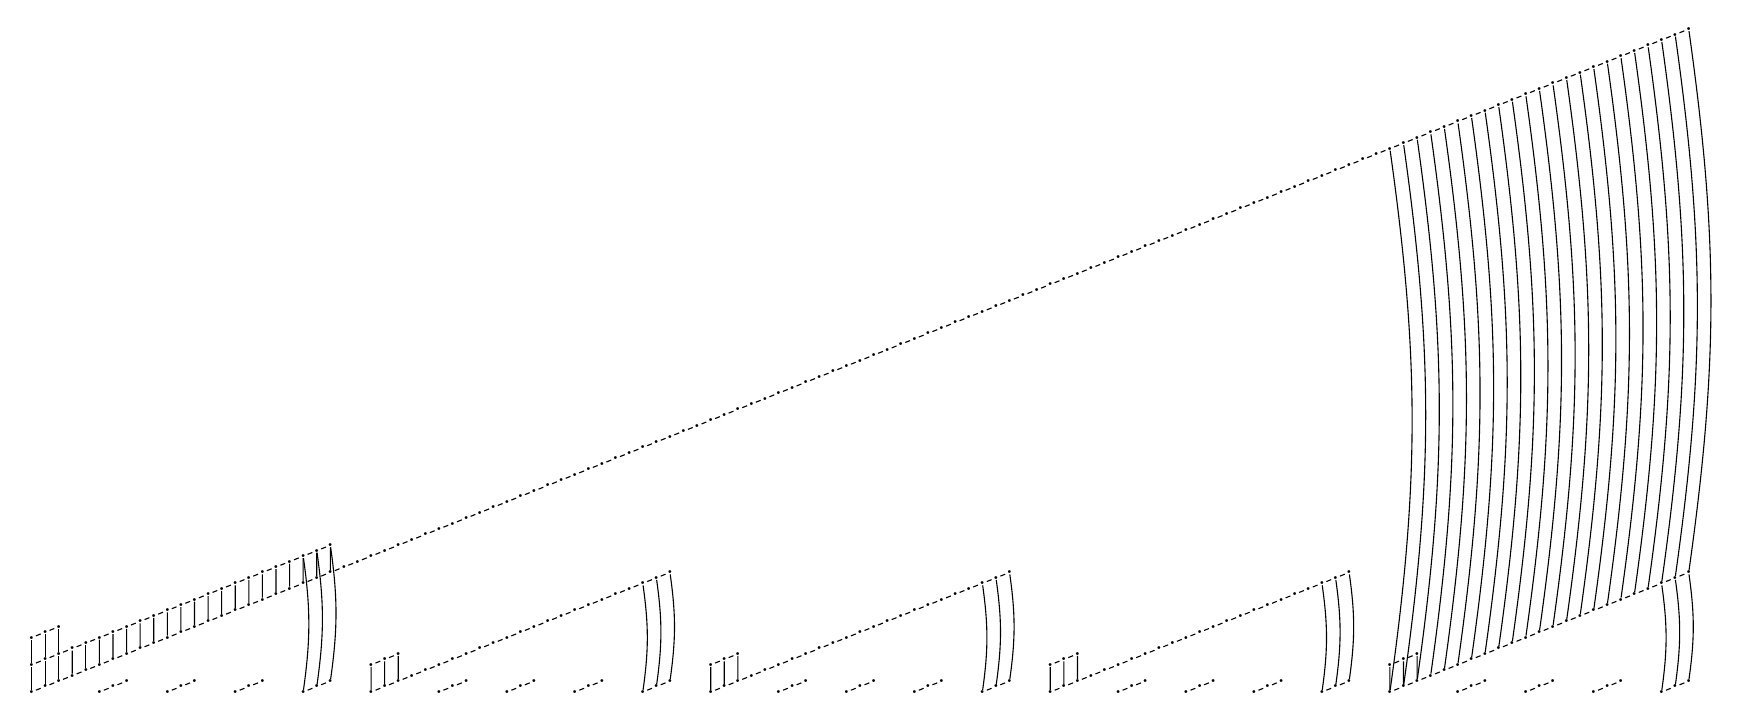
\begin{tikzpicture}[scale=0.345]
\node[inner sep=0pt] (u0p0m125) at (0.0,0.0) {.};
\node[inner sep=0pt] (u1p0m125) at (0.5,0.2) {.};
\node[inner sep=0pt] (u2p0m125) at (1.0,0.4) {.};
\node[inner sep=0pt] (u3p0m125) at (1.5,0.6) {.};
\node[inner sep=0pt] (u4p0m125) at (2.0,0.8) {.};
\node[inner sep=0pt] (u5p0m125) at (2.5,1.0) {.};
\node[inner sep=0pt] (u6p0m125) at (3.0,1.2) {.};
\node[inner sep=0pt] (u7p0m125) at (3.5,1.4) {.};
\node[inner sep=0pt] (u8p0m125) at (4.0,1.6) {.};
\node[inner sep=0pt] (u9p0m125) at (4.5,1.8000001) {.};
\node[inner sep=0pt] (u10p0m125) at (5.0,2.0) {.};
\node[inner sep=0pt] (u11p0m125) at (5.5,2.2) {.};
\node[inner sep=0pt] (u12p0m125) at (6.0,2.4) {.};
\node[inner sep=0pt] (u13p0m125) at (6.5,2.6000001) {.};
\node[inner sep=0pt] (u14p0m125) at (7.0,2.8) {.};
\node[inner sep=0pt] (u15p0m125) at (7.5,3.0) {.};
\node[inner sep=0pt] (u16p0m125) at (8.0,3.2) {.};
\node[inner sep=0pt] (u17p0m125) at (8.5,3.4) {.};
\node[inner sep=0pt] (u18p0m125) at (9.0,3.6000001) {.};
\node[inner sep=0pt] (u19p0m125) at (9.5,3.8) {.};
\node[inner sep=0pt] (u20p0m125) at (10.0,4.0) {.};
\node[inner sep=0pt] (u21p0m125) at (10.5,4.2000003) {.};
\node[inner sep=0pt] (u22p0m125) at (11.0,4.4) {.};
\node[inner sep=0pt] (u23p0m125) at (11.5,4.6) {.};
\node[inner sep=0pt] (u24p0m125) at (12.0,4.8) {.};
\node[inner sep=0pt] (u25p0m125) at (12.5,5.0) {.};
\node[inner sep=0pt] (u26p0m125) at (13.0,5.2000003) {.};
\node[inner sep=0pt] (u27p0m125) at (13.5,5.4) {.};
\node[inner sep=0pt] (u28p0m125) at (14.0,5.6) {.};
\node[inner sep=0pt] (u29p0m125) at (14.5,5.8) {.};
\node[inner sep=0pt] (u30p0m125) at (15.0,6.0) {.};
\node[inner sep=0pt] (u31p0m125) at (15.5,6.2000003) {.};
\node[inner sep=0pt] (u32p0m125) at (16.0,6.4) {.};
\node[inner sep=0pt] (u33p0m125) at (16.5,6.6) {.};
\node[inner sep=0pt] (u34p0m125) at (17.0,6.8) {.};
\node[inner sep=0pt] (u35p0m125) at (17.5,7.0) {.};
\node[inner sep=0pt] (u36p0m125) at (18.0,7.2000003) {.};
\node[inner sep=0pt] (u37p0m125) at (18.5,7.4) {.};
\node[inner sep=0pt] (u38p0m125) at (19.0,7.6) {.};
\node[inner sep=0pt] (u39p0m125) at (19.5,7.8) {.};
\node[inner sep=0pt] (u40p0m125) at (20.0,8.0) {.};
\node[inner sep=0pt] (u41p0m125) at (20.5,8.2) {.};
\node[inner sep=0pt] (u42p0m125) at (21.0,8.400001) {.};
\node[inner sep=0pt] (u43p0m125) at (21.5,8.6) {.};
\node[inner sep=0pt] (u44p0m125) at (22.0,8.8) {.};
\node[inner sep=0pt] (u45p0m125) at (22.5,9.0) {.};
\node[inner sep=0pt] (u46p0m125) at (23.0,9.2) {.};
\node[inner sep=0pt] (u47p0m125) at (23.5,9.400001) {.};
\node[inner sep=0pt] (u48p0m125) at (24.0,9.6) {.};
\node[inner sep=0pt] (u49p0m125) at (24.5,9.8) {.};
\node[inner sep=0pt] (u50p0m125) at (25.0,10.0) {.};
\node[inner sep=0pt] (u51p0m125) at (25.5,10.2) {.};
\node[inner sep=0pt] (u52p0m125) at (26.0,10.400001) {.};
\node[inner sep=0pt] (u53p0m125) at (26.5,10.6) {.};
\node[inner sep=0pt] (u54p0m125) at (27.0,10.8) {.};
\node[inner sep=0pt] (u55p0m125) at (27.5,11.0) {.};
\node[inner sep=0pt] (u56p0m125) at (28.0,11.2) {.};
\node[inner sep=0pt] (u57p0m125) at (28.5,11.400001) {.};
\node[inner sep=0pt] (u58p0m125) at (29.0,11.6) {.};
\node[inner sep=0pt] (u59p0m125) at (29.5,11.8) {.};
\node[inner sep=0pt] (u60p0m125) at (30.0,12.0) {.};
\node[inner sep=0pt] (u61p0m125) at (30.5,12.2) {.};
\node[inner sep=0pt] (u62p0m125) at (31.0,12.400001) {.};
\node[inner sep=0pt] (u63p0m125) at (31.5,12.6) {.};
\node[inner sep=0pt] (u64p0m125) at (32.0,12.8) {.};
\node[inner sep=0pt] (u65p0m125) at (32.5,13.0) {.};
\node[inner sep=0pt] (u66p0m125) at (33.0,13.2) {.};
\node[inner sep=0pt] (u67p0m125) at (33.5,13.400001) {.};
\node[inner sep=0pt] (u68p0m125) at (34.0,13.6) {.};
\node[inner sep=0pt] (u69p0m125) at (34.5,13.8) {.};
\node[inner sep=0pt] (u70p0m125) at (35.0,14.0) {.};
\node[inner sep=0pt] (u71p0m125) at (35.5,14.2) {.};
\node[inner sep=0pt] (u72p0m125) at (36.0,14.400001) {.};
\node[inner sep=0pt] (u73p0m125) at (36.5,14.6) {.};
\node[inner sep=0pt] (u74p0m125) at (37.0,14.8) {.};
\node[inner sep=0pt] (u75p0m125) at (37.5,15.0) {.};
\node[inner sep=0pt] (u76p0m125) at (38.0,15.2) {.};
\node[inner sep=0pt] (u77p0m125) at (38.5,15.400001) {.};
\node[inner sep=0pt] (u78p0m125) at (39.0,15.6) {.};
\node[inner sep=0pt] (u79p0m125) at (39.5,15.8) {.};
\node[inner sep=0pt] (u80p0m125) at (40.0,16.0) {.};
\node[inner sep=0pt] (u81p0m125) at (40.5,16.2) {.};
\node[inner sep=0pt] (u82p0m125) at (41.0,16.4) {.};
\node[inner sep=0pt] (u83p0m125) at (41.5,16.6) {.};
\node[inner sep=0pt] (u84p0m125) at (42.0,16.800001) {.};
\node[inner sep=0pt] (u85p0m125) at (42.5,17.0) {.};
\node[inner sep=0pt] (u86p0m125) at (43.0,17.2) {.};
\node[inner sep=0pt] (u87p0m125) at (43.5,17.4) {.};
\node[inner sep=0pt] (u88p0m125) at (44.0,17.6) {.};
\node[inner sep=0pt] (u89p0m125) at (44.5,17.800001) {.};
\node[inner sep=0pt] (u90p0m125) at (45.0,18.0) {.};
\node[inner sep=0pt] (u91p0m125) at (45.5,18.2) {.};
\node[inner sep=0pt] (u92p0m125) at (46.0,18.4) {.};
\node[inner sep=0pt] (u93p0m125) at (46.5,18.6) {.};
\node[inner sep=0pt] (u94p0m125) at (47.0,18.800001) {.};
\node[inner sep=0pt] (u95p0m125) at (47.5,19.0) {.};
\node[inner sep=0pt] (u96p0m125) at (48.0,19.2) {.};
\node[inner sep=0pt] (u97p0m125) at (48.5,19.4) {.};
\node[inner sep=0pt] (u98p0m125) at (49.0,19.6) {.};
\node[inner sep=0pt] (u99p0m125) at (49.5,19.800001) {.};
\node[inner sep=0pt] (u100p0m125) at (50.0,20.0) {.};
\node[inner sep=0pt] (u101p0m125) at (50.5,20.2) {.};
\node[inner sep=0pt] (u102p0m125) at (51.0,20.4) {.};
\node[inner sep=0pt] (u103p0m125) at (51.5,20.6) {.};
\node[inner sep=0pt] (u104p0m125) at (52.0,20.800001) {.};
\node[inner sep=0pt] (u105p0m125) at (52.5,21.0) {.};
\node[inner sep=0pt] (u106p0m125) at (53.0,21.2) {.};
\node[inner sep=0pt] (u107p0m125) at (53.5,21.4) {.};
\node[inner sep=0pt] (u108p0m125) at (54.0,21.6) {.};
\node[inner sep=0pt] (u109p0m125) at (54.5,21.800001) {.};
\node[inner sep=0pt] (u110p0m125) at (55.0,22.0) {.};
\node[inner sep=0pt] (u111p0m125) at (55.5,22.2) {.};
\node[inner sep=0pt] (u112p0m125) at (56.0,22.4) {.};
\node[inner sep=0pt] (u113p0m125) at (56.5,22.6) {.};
\node[inner sep=0pt] (u114p0m125) at (57.0,22.800001) {.};
\node[inner sep=0pt] (u115p0m125) at (57.5,23.0) {.};
\node[inner sep=0pt] (u116p0m125) at (58.0,23.2) {.};
\node[inner sep=0pt] (u117p0m125) at (58.5,23.4) {.};
\node[inner sep=0pt] (u118p0m125) at (59.0,23.6) {.};
\node[inner sep=0pt] (u119p0m125) at (59.5,23.800001) {.};
\node[inner sep=0pt] (u120p0m125) at (60.0,24.0) {.};
\node[inner sep=0pt] (u121p0m125) at (60.5,24.2) {.};
\node[inner sep=0pt] (u122p0m125) at (61.0,24.4) {.};
\node[inner sep=0pt] (u0p1m125) at (0.0,1.0) {.};
\node[inner sep=0pt] (u1p1m125) at (0.5,1.2) {.};
\node[inner sep=0pt] (u2p1m125) at (1.0,1.4) {.};
\node[inner sep=0pt] (u3p1m125) at (1.5,1.6) {.};
\node[inner sep=0pt] (u4p1m125) at (2.0,1.8) {.};
\node[inner sep=0pt] (u5p1m125) at (2.5,2.0) {.};
\node[inner sep=0pt] (u6p1m125) at (3.0,2.2) {.};
\node[inner sep=0pt] (u7p1m125) at (3.5,2.4) {.};
\node[inner sep=0pt] (u8p1m125) at (4.0,2.6) {.};
\node[inner sep=0pt] (u9p1m125) at (4.5,2.8000002) {.};
\node[inner sep=0pt] (u10p1m125) at (5.0,3.0) {.};
\node[inner sep=0pt] (u11p1m125) at (5.5,3.2) {.};
\node[inner sep=0pt] (u12p1m125) at (6.0,3.4) {.};
\node[inner sep=0pt] (u13p1m125) at (6.5,3.6000001) {.};
\node[inner sep=0pt] (u14p1m125) at (7.0,3.8) {.};
\node[inner sep=0pt] (u15p1m125) at (7.5,4.0) {.};
\node[inner sep=0pt] (u16p1m125) at (8.0,4.2) {.};
\node[inner sep=0pt] (u17p1m125) at (8.5,4.4) {.};
\node[inner sep=0pt] (u18p1m125) at (9.0,4.6000004) {.};
\node[inner sep=0pt] (u19p1m125) at (9.5,4.8) {.};
\node[inner sep=0pt] (u20p1m125) at (10.0,5.0) {.};
\node[inner sep=0pt] (u21p1m125) at (10.5,5.2000003) {.};
\node[inner sep=0pt] (u22p1m125) at (11.0,5.4) {.};
\node[inner sep=0pt] (u0p2m125) at (0.0,2.0) {.};
\node[inner sep=0pt] (u1p2m125) at (0.5,2.2) {.};
\node[inner sep=0pt] (u2p2m125) at (1.0,2.4) {.};
\node[inner sep=0pt] (u0p0m130) at (2.5,0.0) {.};
\node[inner sep=0pt] (u1p0m130) at (3.0,0.2) {.};
\node[inner sep=0pt] (u2p0m130) at (3.5,0.4) {.};
\node[inner sep=0pt] (u0p0m135) at (5.0,0.0) {.};
\node[inner sep=0pt] (u1p0m135) at (5.5,0.2) {.};
\node[inner sep=0pt] (u2p0m135) at (6.0,0.4) {.};
\node[inner sep=0pt] (u0p0m140) at (7.5,0.0) {.};
\node[inner sep=0pt] (u1p0m140) at (8.0,0.2) {.};
\node[inner sep=0pt] (u2p0m140) at (8.5,0.4) {.};
\node[inner sep=0pt] (u0p0m145) at (10.0,0.0) {.};
\node[inner sep=0pt] (u1p0m145) at (10.5,0.2) {.};
\node[inner sep=0pt] (u2p0m145) at (11.0,0.4) {.};
\node[inner sep=0pt] (u0p0m150) at (12.5,0.0) {.};
\node[inner sep=0pt] (u1p0m150) at (13.0,0.2) {.};
\node[inner sep=0pt] (u2p0m150) at (13.5,0.4) {.};
\node[inner sep=0pt] (u3p0m150) at (14.0,0.6) {.};
\node[inner sep=0pt] (u4p0m150) at (14.5,0.8) {.};
\node[inner sep=0pt] (u5p0m150) at (15.0,1.0) {.};
\node[inner sep=0pt] (u6p0m150) at (15.5,1.2) {.};
\node[inner sep=0pt] (u7p0m150) at (16.0,1.4) {.};
\node[inner sep=0pt] (u8p0m150) at (16.5,1.6) {.};
\node[inner sep=0pt] (u9p0m150) at (17.0,1.8000001) {.};
\node[inner sep=0pt] (u10p0m150) at (17.5,2.0) {.};
\node[inner sep=0pt] (u11p0m150) at (18.0,2.2) {.};
\node[inner sep=0pt] (u12p0m150) at (18.5,2.4) {.};
\node[inner sep=0pt] (u13p0m150) at (19.0,2.6000001) {.};
\node[inner sep=0pt] (u14p0m150) at (19.5,2.8) {.};
\node[inner sep=0pt] (u15p0m150) at (20.0,3.0) {.};
\node[inner sep=0pt] (u16p0m150) at (20.5,3.2) {.};
\node[inner sep=0pt] (u17p0m150) at (21.0,3.4) {.};
\node[inner sep=0pt] (u18p0m150) at (21.5,3.6000001) {.};
\node[inner sep=0pt] (u19p0m150) at (22.0,3.8) {.};
\node[inner sep=0pt] (u20p0m150) at (22.5,4.0) {.};
\node[inner sep=0pt] (u21p0m150) at (23.0,4.2000003) {.};
\node[inner sep=0pt] (u22p0m150) at (23.5,4.4) {.};
\node[inner sep=0pt] (u0p1m150) at (12.5,1.0) {.};
\node[inner sep=0pt] (u1p1m150) at (13.0,1.2) {.};
\node[inner sep=0pt] (u2p1m150) at (13.5,1.4) {.};
\node[inner sep=0pt] (u0p0m155) at (15.0,0.0) {.};
\node[inner sep=0pt] (u1p0m155) at (15.5,0.2) {.};
\node[inner sep=0pt] (u2p0m155) at (16.0,0.4) {.};
\node[inner sep=0pt] (u0p0m160) at (17.5,0.0) {.};
\node[inner sep=0pt] (u1p0m160) at (18.0,0.2) {.};
\node[inner sep=0pt] (u2p0m160) at (18.5,0.4) {.};
\node[inner sep=0pt] (u0p0m165) at (20.0,0.0) {.};
\node[inner sep=0pt] (u1p0m165) at (20.5,0.2) {.};
\node[inner sep=0pt] (u2p0m165) at (21.0,0.4) {.};
\node[inner sep=0pt] (u0p0m170) at (22.5,0.0) {.};
\node[inner sep=0pt] (u1p0m170) at (23.0,0.2) {.};
\node[inner sep=0pt] (u2p0m170) at (23.5,0.4) {.};
\node[inner sep=0pt] (u0p0m175) at (25.0,0.0) {.};
\node[inner sep=0pt] (u1p0m175) at (25.5,0.2) {.};
\node[inner sep=0pt] (u2p0m175) at (26.0,0.4) {.};
\node[inner sep=0pt] (u3p0m175) at (26.5,0.6) {.};
\node[inner sep=0pt] (u4p0m175) at (27.0,0.8) {.};
\node[inner sep=0pt] (u5p0m175) at (27.5,1.0) {.};
\node[inner sep=0pt] (u6p0m175) at (28.0,1.2) {.};
\node[inner sep=0pt] (u7p0m175) at (28.5,1.4) {.};
\node[inner sep=0pt] (u8p0m175) at (29.0,1.6) {.};
\node[inner sep=0pt] (u9p0m175) at (29.5,1.8000001) {.};
\node[inner sep=0pt] (u10p0m175) at (30.0,2.0) {.};
\node[inner sep=0pt] (u11p0m175) at (30.5,2.2) {.};
\node[inner sep=0pt] (u12p0m175) at (31.0,2.4) {.};
\node[inner sep=0pt] (u13p0m175) at (31.5,2.6000001) {.};
\node[inner sep=0pt] (u14p0m175) at (32.0,2.8) {.};
\node[inner sep=0pt] (u15p0m175) at (32.5,3.0) {.};
\node[inner sep=0pt] (u16p0m175) at (33.0,3.2) {.};
\node[inner sep=0pt] (u17p0m175) at (33.5,3.4) {.};
\node[inner sep=0pt] (u18p0m175) at (34.0,3.6000001) {.};
\node[inner sep=0pt] (u19p0m175) at (34.5,3.8) {.};
\node[inner sep=0pt] (u20p0m175) at (35.0,4.0) {.};
\node[inner sep=0pt] (u21p0m175) at (35.5,4.2000003) {.};
\node[inner sep=0pt] (u22p0m175) at (36.0,4.4) {.};
\node[inner sep=0pt] (u0p1m175) at (25.0,1.0) {.};
\node[inner sep=0pt] (u1p1m175) at (25.5,1.2) {.};
\node[inner sep=0pt] (u2p1m175) at (26.0,1.4) {.};
\node[inner sep=0pt] (u0p0m180) at (27.5,0.0) {.};
\node[inner sep=0pt] (u1p0m180) at (28.0,0.2) {.};
\node[inner sep=0pt] (u2p0m180) at (28.5,0.4) {.};
\node[inner sep=0pt] (u0p0m185) at (30.0,0.0) {.};
\node[inner sep=0pt] (u1p0m185) at (30.5,0.2) {.};
\node[inner sep=0pt] (u2p0m185) at (31.0,0.4) {.};
\node[inner sep=0pt] (u0p0m190) at (32.5,0.0) {.};
\node[inner sep=0pt] (u1p0m190) at (33.0,0.2) {.};
\node[inner sep=0pt] (u2p0m190) at (33.5,0.4) {.};
\node[inner sep=0pt] (u0p0m195) at (35.0,0.0) {.};
\node[inner sep=0pt] (u1p0m195) at (35.5,0.2) {.};
\node[inner sep=0pt] (u2p0m195) at (36.0,0.4) {.};
\node[inner sep=0pt] (u0p0m200) at (37.5,0.0) {.};
\node[inner sep=0pt] (u1p0m200) at (38.0,0.2) {.};
\node[inner sep=0pt] (u2p0m200) at (38.5,0.4) {.};
\node[inner sep=0pt] (u3p0m200) at (39.0,0.6) {.};
\node[inner sep=0pt] (u4p0m200) at (39.5,0.8) {.};
\node[inner sep=0pt] (u5p0m200) at (40.0,1.0) {.};
\node[inner sep=0pt] (u6p0m200) at (40.5,1.2) {.};
\node[inner sep=0pt] (u7p0m200) at (41.0,1.4) {.};
\node[inner sep=0pt] (u8p0m200) at (41.5,1.6) {.};
\node[inner sep=0pt] (u9p0m200) at (42.0,1.8000001) {.};
\node[inner sep=0pt] (u10p0m200) at (42.5,2.0) {.};
\node[inner sep=0pt] (u11p0m200) at (43.0,2.2) {.};
\node[inner sep=0pt] (u12p0m200) at (43.5,2.4) {.};
\node[inner sep=0pt] (u13p0m200) at (44.0,2.6000001) {.};
\node[inner sep=0pt] (u14p0m200) at (44.5,2.8) {.};
\node[inner sep=0pt] (u15p0m200) at (45.0,3.0) {.};
\node[inner sep=0pt] (u16p0m200) at (45.5,3.2) {.};
\node[inner sep=0pt] (u17p0m200) at (46.0,3.4) {.};
\node[inner sep=0pt] (u18p0m200) at (46.5,3.6000001) {.};
\node[inner sep=0pt] (u19p0m200) at (47.0,3.8) {.};
\node[inner sep=0pt] (u20p0m200) at (47.5,4.0) {.};
\node[inner sep=0pt] (u21p0m200) at (48.0,4.2000003) {.};
\node[inner sep=0pt] (u22p0m200) at (48.5,4.4) {.};
\node[inner sep=0pt] (u0p1m200) at (37.5,1.0) {.};
\node[inner sep=0pt] (u1p1m200) at (38.0,1.2) {.};
\node[inner sep=0pt] (u2p1m200) at (38.5,1.4) {.};
\node[inner sep=0pt] (u0p0m205) at (40.0,0.0) {.};
\node[inner sep=0pt] (u1p0m205) at (40.5,0.2) {.};
\node[inner sep=0pt] (u2p0m205) at (41.0,0.4) {.};
\node[inner sep=0pt] (u0p0m210) at (42.5,0.0) {.};
\node[inner sep=0pt] (u1p0m210) at (43.0,0.2) {.};
\node[inner sep=0pt] (u2p0m210) at (43.5,0.4) {.};
\node[inner sep=0pt] (u0p0m215) at (45.0,0.0) {.};
\node[inner sep=0pt] (u1p0m215) at (45.5,0.2) {.};
\node[inner sep=0pt] (u2p0m215) at (46.0,0.4) {.};
\node[inner sep=0pt] (u0p0m220) at (47.5,0.0) {.};
\node[inner sep=0pt] (u1p0m220) at (48.0,0.2) {.};
\node[inner sep=0pt] (u2p0m220) at (48.5,0.4) {.};
\node[inner sep=0pt] (u0p0m225) at (50.0,0.0) {.};
\node[inner sep=0pt] (u1p0m225) at (50.5,0.2) {.};
\node[inner sep=0pt] (u2p0m225) at (51.0,0.4) {.};
\node[inner sep=0pt] (u3p0m225) at (51.5,0.6) {.};
\node[inner sep=0pt] (u4p0m225) at (52.0,0.8) {.};
\node[inner sep=0pt] (u5p0m225) at (52.5,1.0) {.};
\node[inner sep=0pt] (u6p0m225) at (53.0,1.2) {.};
\node[inner sep=0pt] (u7p0m225) at (53.5,1.4) {.};
\node[inner sep=0pt] (u8p0m225) at (54.0,1.6) {.};
\node[inner sep=0pt] (u9p0m225) at (54.5,1.8000001) {.};
\node[inner sep=0pt] (u10p0m225) at (55.0,2.0) {.};
\node[inner sep=0pt] (u11p0m225) at (55.5,2.2) {.};
\node[inner sep=0pt] (u12p0m225) at (56.0,2.4) {.};
\node[inner sep=0pt] (u13p0m225) at (56.5,2.6000001) {.};
\node[inner sep=0pt] (u14p0m225) at (57.0,2.8) {.};
\node[inner sep=0pt] (u15p0m225) at (57.5,3.0) {.};
\node[inner sep=0pt] (u16p0m225) at (58.0,3.2) {.};
\node[inner sep=0pt] (u17p0m225) at (58.5,3.4) {.};
\node[inner sep=0pt] (u18p0m225) at (59.0,3.6000001) {.};
\node[inner sep=0pt] (u19p0m225) at (59.5,3.8) {.};
\node[inner sep=0pt] (u20p0m225) at (60.0,4.0) {.};
\node[inner sep=0pt] (u21p0m225) at (60.5,4.2000003) {.};
\node[inner sep=0pt] (u22p0m225) at (61.0,4.4) {.};
\node[inner sep=0pt] (u0p1m225) at (50.0,1.0) {.};
\node[inner sep=0pt] (u1p1m225) at (50.5,1.2) {.};
\node[inner sep=0pt] (u2p1m225) at (51.0,1.4) {.};
\node[inner sep=0pt] (u0p0m230) at (52.5,0.0) {.};
\node[inner sep=0pt] (u1p0m230) at (53.0,0.2) {.};
\node[inner sep=0pt] (u2p0m230) at (53.5,0.4) {.};
\node[inner sep=0pt] (u0p0m235) at (55.0,0.0) {.};
\node[inner sep=0pt] (u1p0m235) at (55.5,0.2) {.};
\node[inner sep=0pt] (u2p0m235) at (56.0,0.4) {.};
\node[inner sep=0pt] (u0p0m240) at (57.5,0.0) {.};
\node[inner sep=0pt] (u1p0m240) at (58.0,0.2) {.};
\node[inner sep=0pt] (u2p0m240) at (58.5,0.4) {.};
\node[inner sep=0pt] (u0p0m245) at (60.0,0.0) {.};
\node[inner sep=0pt] (u1p0m245) at (60.5,0.2) {.};
\node[inner sep=0pt] (u2p0m245) at (61.0,0.4) {.};
\draw (u0p0m125) to (u1p0m125);
\draw (u0p0m125) to (u0p1m125);
\draw (u1p0m125) to (u2p0m125);
\draw (u1p0m125) to (u1p1m125);
\draw (u2p0m125) to (u3p0m125);
\draw (u2p0m125) to (u2p1m125);
\draw (u3p0m125) to (u4p0m125);
\draw (u3p0m125) to (u3p1m125);
\draw (u4p0m125) to (u5p0m125);
\draw (u4p0m125) to (u4p1m125);
\draw (u5p0m125) to (u6p0m125);
\draw (u5p0m125) to (u5p1m125);
\draw (u6p0m125) to (u7p0m125);
\draw (u6p0m125) to (u6p1m125);
\draw (u7p0m125) to (u8p0m125);
\draw (u7p0m125) to (u7p1m125);
\draw (u8p0m125) to (u9p0m125);
\draw (u8p0m125) to (u8p1m125);
\draw (u9p0m125) to (u10p0m125);
\draw (u9p0m125) to (u9p1m125);
\draw (u10p0m125) to (u11p0m125);
\draw (u10p0m125) to (u10p1m125);
\draw (u11p0m125) to (u12p0m125);
\draw (u11p0m125) to (u11p1m125);
\draw (u12p0m125) to (u13p0m125);
\draw (u12p0m125) to (u12p1m125);
\draw (u13p0m125) to (u14p0m125);
\draw (u13p0m125) to (u13p1m125);
\draw (u14p0m125) to (u15p0m125);
\draw (u14p0m125) to (u14p1m125);
\draw (u15p0m125) to (u16p0m125);
\draw (u15p0m125) to (u15p1m125);
\draw (u16p0m125) to (u17p0m125);
\draw (u16p0m125) to (u16p1m125);
\draw (u17p0m125) to (u18p0m125);
\draw (u17p0m125) to (u17p1m125);
\draw (u18p0m125) to (u19p0m125);
\draw (u18p0m125) to (u18p1m125);
\draw (u19p0m125) to (u20p0m125);
\draw (u19p0m125) to (u19p1m125);
\draw (u20p0m125) to (u21p0m125);
\draw (u20p0m125) to (u20p1m125);
\draw (u21p0m125) to (u22p0m125);
\draw (u21p0m125) to (u21p1m125);
\draw (u22p0m125) to (u23p0m125);
\draw (u22p0m125) to (u22p1m125);
\draw (u23p0m125) to (u24p0m125);
\draw (u24p0m125) to (u25p0m125);
\draw (u25p0m125) to (u26p0m125);
\draw (u26p0m125) to (u27p0m125);
\draw (u27p0m125) to (u28p0m125);
\draw (u28p0m125) to (u29p0m125);
\draw (u29p0m125) to (u30p0m125);
\draw (u30p0m125) to (u31p0m125);
\draw (u31p0m125) to (u32p0m125);
\draw (u32p0m125) to (u33p0m125);
\draw (u33p0m125) to (u34p0m125);
\draw (u34p0m125) to (u35p0m125);
\draw (u35p0m125) to (u36p0m125);
\draw (u36p0m125) to (u37p0m125);
\draw (u37p0m125) to (u38p0m125);
\draw (u38p0m125) to (u39p0m125);
\draw (u39p0m125) to (u40p0m125);
\draw (u40p0m125) to (u41p0m125);
\draw (u41p0m125) to (u42p0m125);
\draw (u42p0m125) to (u43p0m125);
\draw (u43p0m125) to (u44p0m125);
\draw (u44p0m125) to (u45p0m125);
\draw (u45p0m125) to (u46p0m125);
\draw (u46p0m125) to (u47p0m125);
\draw (u47p0m125) to (u48p0m125);
\draw (u48p0m125) to (u49p0m125);
\draw (u49p0m125) to (u50p0m125);
\draw (u50p0m125) to (u51p0m125);
\draw (u51p0m125) to (u52p0m125);
\draw (u52p0m125) to (u53p0m125);
\draw (u53p0m125) to (u54p0m125);
\draw (u54p0m125) to (u55p0m125);
\draw (u55p0m125) to (u56p0m125);
\draw (u56p0m125) to (u57p0m125);
\draw (u57p0m125) to (u58p0m125);
\draw (u58p0m125) to (u59p0m125);
\draw (u59p0m125) to (u60p0m125);
\draw (u60p0m125) to (u61p0m125);
\draw (u61p0m125) to (u62p0m125);
\draw (u62p0m125) to (u63p0m125);
\draw (u63p0m125) to (u64p0m125);
\draw (u64p0m125) to (u65p0m125);
\draw (u65p0m125) to (u66p0m125);
\draw (u66p0m125) to (u67p0m125);
\draw (u67p0m125) to (u68p0m125);
\draw (u68p0m125) to (u69p0m125);
\draw (u69p0m125) to (u70p0m125);
\draw (u70p0m125) to (u71p0m125);
\draw (u71p0m125) to (u72p0m125);
\draw (u72p0m125) to (u73p0m125);
\draw (u73p0m125) to (u74p0m125);
\draw (u74p0m125) to (u75p0m125);
\draw (u75p0m125) to (u76p0m125);
\draw (u76p0m125) to (u77p0m125);
\draw (u77p0m125) to (u78p0m125);
\draw (u78p0m125) to (u79p0m125);
\draw (u79p0m125) to (u80p0m125);
\draw (u80p0m125) to (u81p0m125);
\draw (u81p0m125) to (u82p0m125);
\draw (u82p0m125) to (u83p0m125);
\draw (u83p0m125) to (u84p0m125);
\draw (u84p0m125) to (u85p0m125);
\draw (u85p0m125) to (u86p0m125);
\draw (u86p0m125) to (u87p0m125);
\draw (u87p0m125) to (u88p0m125);
\draw (u88p0m125) to (u89p0m125);
\draw (u89p0m125) to (u90p0m125);
\draw (u90p0m125) to (u91p0m125);
\draw (u91p0m125) to (u92p0m125);
\draw (u92p0m125) to (u93p0m125);
\draw (u93p0m125) to (u94p0m125);
\draw (u94p0m125) to (u95p0m125);
\draw (u95p0m125) to (u96p0m125);
\draw (u96p0m125) to (u97p0m125);
\draw (u97p0m125) to (u98p0m125);
\draw (u98p0m125) to (u99p0m125);
\draw (u99p0m125) to (u100p0m125);
\draw (u100p0m125) to (u101p0m125);
\draw (u101p0m125) to (u102p0m125);
\draw (u102p0m125) to (u103p0m125);
\draw (u103p0m125) to (u104p0m125);
\draw (u104p0m125) to (u105p0m125);
\draw (u105p0m125) to (u106p0m125);
\draw (u106p0m125) to (u107p0m125);
\draw (u107p0m125) to (u108p0m125);
\draw (u108p0m125) to (u109p0m125);
\draw (u109p0m125) to (u110p0m125);
\draw (u110p0m125) to (u111p0m125);
\draw (u111p0m125) to (u112p0m125);
\draw (u112p0m125) to (u113p0m125);
\draw (u113p0m125) to (u114p0m125);
\draw (u114p0m125) to (u115p0m125);
\draw (u115p0m125) to (u116p0m125);
\draw (u116p0m125) to (u117p0m125);
\draw (u117p0m125) to (u118p0m125);
\draw (u118p0m125) to (u119p0m125);
\draw (u119p0m125) to (u120p0m125);
\draw (u120p0m125) to (u121p0m125);
\draw (u121p0m125) to (u122p0m125);
\draw (u0p1m125) to (u1p1m125);
\draw (u0p1m125) to (u0p2m125);
\draw (u1p1m125) to (u2p1m125);
\draw (u1p1m125) to (u1p2m125);
\draw (u2p1m125) to (u3p1m125);
\draw (u2p1m125) to (u2p2m125);
\draw (u3p1m125) to (u4p1m125);
\draw (u4p1m125) to (u5p1m125);
\draw (u5p1m125) to (u6p1m125);
\draw (u6p1m125) to (u7p1m125);
\draw (u7p1m125) to (u8p1m125);
\draw (u8p1m125) to (u9p1m125);
\draw (u9p1m125) to (u10p1m125);
\draw (u10p1m125) to (u11p1m125);
\draw (u11p1m125) to (u12p1m125);
\draw (u12p1m125) to (u13p1m125);
\draw (u13p1m125) to (u14p1m125);
\draw (u14p1m125) to (u15p1m125);
\draw (u15p1m125) to (u16p1m125);
\draw (u16p1m125) to (u17p1m125);
\draw (u17p1m125) to (u18p1m125);
\draw (u18p1m125) to (u19p1m125);
\draw (u19p1m125) to (u20p1m125);
\draw (u20p1m125) to (u21p1m125);
\draw (u21p1m125) to (u22p1m125);
\draw (u0p2m125) to (u1p2m125);
\draw (u1p2m125) to (u2p2m125);
\draw (u0p0m130) to (u1p0m130);
\draw (u1p0m130) to (u2p0m130);
\draw (u0p0m135) to (u1p0m135);
\draw (u1p0m135) to (u2p0m135);
\draw (u0p0m140) to (u1p0m140);
\draw (u1p0m140) to (u2p0m140);
\draw (u0p0m145) to (u1p0m145);
\draw (u0p0m145) to[bend right=8] (u20p1m125);
\draw (u1p0m145) to (u2p0m145);
\draw (u1p0m145) to[bend right=8] (u21p1m125);
\draw (u2p0m145) to[bend right=8] (u22p1m125);
\draw (u0p0m150) to (u1p0m150);
\draw (u0p0m150) to (u0p1m150);
\draw (u1p0m150) to (u2p0m150);
\draw (u1p0m150) to (u1p1m150);
\draw (u2p0m150) to (u3p0m150);
\draw (u2p0m150) to (u2p1m150);
\draw (u3p0m150) to (u4p0m150);
\draw (u4p0m150) to (u5p0m150);
\draw (u5p0m150) to (u6p0m150);
\draw (u6p0m150) to (u7p0m150);
\draw (u7p0m150) to (u8p0m150);
\draw (u8p0m150) to (u9p0m150);
\draw (u9p0m150) to (u10p0m150);
\draw (u10p0m150) to (u11p0m150);
\draw (u11p0m150) to (u12p0m150);
\draw (u12p0m150) to (u13p0m150);
\draw (u13p0m150) to (u14p0m150);
\draw (u14p0m150) to (u15p0m150);
\draw (u15p0m150) to (u16p0m150);
\draw (u16p0m150) to (u17p0m150);
\draw (u17p0m150) to (u18p0m150);
\draw (u18p0m150) to (u19p0m150);
\draw (u19p0m150) to (u20p0m150);
\draw (u20p0m150) to (u21p0m150);
\draw (u21p0m150) to (u22p0m150);
\draw (u0p1m150) to (u1p1m150);
\draw (u1p1m150) to (u2p1m150);
\draw (u0p0m155) to (u1p0m155);
\draw (u1p0m155) to (u2p0m155);
\draw (u0p0m160) to (u1p0m160);
\draw (u1p0m160) to (u2p0m160);
\draw (u0p0m165) to (u1p0m165);
\draw (u1p0m165) to (u2p0m165);
\draw (u0p0m170) to (u1p0m170);
\draw (u0p0m170) to[bend right=8] (u20p0m150);
\draw (u1p0m170) to (u2p0m170);
\draw (u1p0m170) to[bend right=8] (u21p0m150);
\draw (u2p0m170) to[bend right=8] (u22p0m150);
\draw (u0p0m175) to (u1p0m175);
\draw (u0p0m175) to (u0p1m175);
\draw (u1p0m175) to (u2p0m175);
\draw (u1p0m175) to (u1p1m175);
\draw (u2p0m175) to (u3p0m175);
\draw (u2p0m175) to (u2p1m175);
\draw (u3p0m175) to (u4p0m175);
\draw (u4p0m175) to (u5p0m175);
\draw (u5p0m175) to (u6p0m175);
\draw (u6p0m175) to (u7p0m175);
\draw (u7p0m175) to (u8p0m175);
\draw (u8p0m175) to (u9p0m175);
\draw (u9p0m175) to (u10p0m175);
\draw (u10p0m175) to (u11p0m175);
\draw (u11p0m175) to (u12p0m175);
\draw (u12p0m175) to (u13p0m175);
\draw (u13p0m175) to (u14p0m175);
\draw (u14p0m175) to (u15p0m175);
\draw (u15p0m175) to (u16p0m175);
\draw (u16p0m175) to (u17p0m175);
\draw (u17p0m175) to (u18p0m175);
\draw (u18p0m175) to (u19p0m175);
\draw (u19p0m175) to (u20p0m175);
\draw (u20p0m175) to (u21p0m175);
\draw (u21p0m175) to (u22p0m175);
\draw (u0p1m175) to (u1p1m175);
\draw (u1p1m175) to (u2p1m175);
\draw (u0p0m180) to (u1p0m180);
\draw (u1p0m180) to (u2p0m180);
\draw (u0p0m185) to (u1p0m185);
\draw (u1p0m185) to (u2p0m185);
\draw (u0p0m190) to (u1p0m190);
\draw (u1p0m190) to (u2p0m190);
\draw (u0p0m195) to (u1p0m195);
\draw (u0p0m195) to[bend right=8] (u20p0m175);
\draw (u1p0m195) to (u2p0m195);
\draw (u1p0m195) to[bend right=8] (u21p0m175);
\draw (u2p0m195) to[bend right=8] (u22p0m175);
\draw (u0p0m200) to (u1p0m200);
\draw (u0p0m200) to (u0p1m200);
\draw (u1p0m200) to (u2p0m200);
\draw (u1p0m200) to (u1p1m200);
\draw (u2p0m200) to (u3p0m200);
\draw (u2p0m200) to (u2p1m200);
\draw (u3p0m200) to (u4p0m200);
\draw (u4p0m200) to (u5p0m200);
\draw (u5p0m200) to (u6p0m200);
\draw (u6p0m200) to (u7p0m200);
\draw (u7p0m200) to (u8p0m200);
\draw (u8p0m200) to (u9p0m200);
\draw (u9p0m200) to (u10p0m200);
\draw (u10p0m200) to (u11p0m200);
\draw (u11p0m200) to (u12p0m200);
\draw (u12p0m200) to (u13p0m200);
\draw (u13p0m200) to (u14p0m200);
\draw (u14p0m200) to (u15p0m200);
\draw (u15p0m200) to (u16p0m200);
\draw (u16p0m200) to (u17p0m200);
\draw (u17p0m200) to (u18p0m200);
\draw (u18p0m200) to (u19p0m200);
\draw (u19p0m200) to (u20p0m200);
\draw (u20p0m200) to (u21p0m200);
\draw (u21p0m200) to (u22p0m200);
\draw (u0p1m200) to (u1p1m200);
\draw (u1p1m200) to (u2p1m200);
\draw (u0p0m205) to (u1p0m205);
\draw (u1p0m205) to (u2p0m205);
\draw (u0p0m210) to (u1p0m210);
\draw (u1p0m210) to (u2p0m210);
\draw (u0p0m215) to (u1p0m215);
\draw (u1p0m215) to (u2p0m215);
\draw (u0p0m220) to (u1p0m220);
\draw (u0p0m220) to[bend right=8] (u20p0m200);
\draw (u1p0m220) to (u2p0m220);
\draw (u1p0m220) to[bend right=8] (u21p0m200);
\draw (u2p0m220) to[bend right=8] (u22p0m200);
\draw (u0p0m225) to (u1p0m225);
\draw (u0p0m225) to (u0p1m225);
\draw (u0p0m225) to[bend right=8] (u100p0m125);
\draw (u1p0m225) to (u2p0m225);
\draw (u1p0m225) to (u1p1m225);
\draw (u1p0m225) to[bend right=8] (u101p0m125);
\draw (u2p0m225) to (u3p0m225);
\draw (u2p0m225) to (u2p1m225);
\draw (u2p0m225) to[bend right=8] (u102p0m125);
\draw (u3p0m225) to (u4p0m225);
\draw (u3p0m225) to[bend right=8] (u103p0m125);
\draw (u4p0m225) to (u5p0m225);
\draw (u4p0m225) to[bend right=8] (u104p0m125);
\draw (u5p0m225) to (u6p0m225);
\draw (u5p0m225) to[bend right=8] (u105p0m125);
\draw (u6p0m225) to (u7p0m225);
\draw (u6p0m225) to[bend right=8] (u106p0m125);
\draw (u7p0m225) to (u8p0m225);
\draw (u7p0m225) to[bend right=8] (u107p0m125);
\draw (u8p0m225) to (u9p0m225);
\draw (u8p0m225) to[bend right=8] (u108p0m125);
\draw (u9p0m225) to (u10p0m225);
\draw (u9p0m225) to[bend right=8] (u109p0m125);
\draw (u10p0m225) to (u11p0m225);
\draw (u10p0m225) to[bend right=8] (u110p0m125);
\draw (u11p0m225) to (u12p0m225);
\draw (u11p0m225) to[bend right=8] (u111p0m125);
\draw (u12p0m225) to (u13p0m225);
\draw (u12p0m225) to[bend right=8] (u112p0m125);
\draw (u13p0m225) to (u14p0m225);
\draw (u13p0m225) to[bend right=8] (u113p0m125);
\draw (u14p0m225) to (u15p0m225);
\draw (u14p0m225) to[bend right=8] (u114p0m125);
\draw (u15p0m225) to (u16p0m225);
\draw (u15p0m225) to[bend right=8] (u115p0m125);
\draw (u16p0m225) to (u17p0m225);
\draw (u16p0m225) to[bend right=8] (u116p0m125);
\draw (u17p0m225) to (u18p0m225);
\draw (u17p0m225) to[bend right=8] (u117p0m125);
\draw (u18p0m225) to (u19p0m225);
\draw (u18p0m225) to[bend right=8] (u118p0m125);
\draw (u19p0m225) to (u20p0m225);
\draw (u19p0m225) to[bend right=8] (u119p0m125);
\draw (u20p0m225) to (u21p0m225);
\draw (u20p0m225) to[bend right=8] (u120p0m125);
\draw (u21p0m225) to (u22p0m225);
\draw (u21p0m225) to[bend right=8] (u121p0m125);
\draw (u22p0m225) to[bend right=8] (u122p0m125);
\draw (u0p1m225) to (u1p1m225);
\draw (u1p1m225) to (u2p1m225);
\draw (u0p0m230) to (u1p0m230);
\draw (u1p0m230) to (u2p0m230);
\draw (u0p0m235) to (u1p0m235);
\draw (u1p0m235) to (u2p0m235);
\draw (u0p0m240) to (u1p0m240);
\draw (u1p0m240) to (u2p0m240);
\draw (u0p0m245) to (u1p0m245);
\draw (u0p0m245) to[bend right=8] (u20p0m225);
\draw (u1p0m245) to (u2p0m245);
\draw (u1p0m245) to[bend right=8] (u21p0m225);
\draw (u2p0m245) to[bend right=8] (u22p0m225);
\end{tikzpicture}
  \caption{$T_3$ for $p=5$.}
  \label{fig:p5T3}
\end{sidewaysfigure}


%
%
%
%


We can see that $\THH_*(ku)$ is not $\THH_*(\ell)$ \emph{étale}, by which we mean that
\begin{equation}
  \THH_*(ku) \neq ku_* \otimes_{\ell_*} \THH_*(\ell).
\end{equation}
The extensions of scalars, however, does yield an injection, and in fact a short exact sequence
\begin{equation}
  \begin{tikzcd}
    0 \rar & ku_*\otimes_{\ell_*} \THH_*(\ell) \rar & \THH_*(ku) \rar & \mathcal{C} \rar & 0
  \end{tikzcd}
\end{equation}
where the cokernel $\mathcal{C}$ can be presented as the quotient of the $\Z_{(p)}[u]$-module
\begin{equation}
  P_{p-2}(u)\otimes \Z_{(p)}\{1,\,\sigma u,\,\sigma u\mu_{ap^n},\, n\geq 1,\, a\geq 1,\, \mbox{$a$ not divisible by $p$}\}
\end{equation}
by the relation $p^{n} \sigma u \mu_{ap^n} = 0$ for any $a$ and $n$, $a$ not divisible by $p$.


%
%
%
%
